\chapter{Overview and Integration of Large Language Models}
\label{cha:Introduction_to_the_used_Large_Language_Models}
\textbf{Author:} Luna Schätzle

For the Diploma thesis, there are many different AI models that are in use, such as:
\begin{itemize}
    \item LLMs (Large Language Models)
    \item Diffusion Models (Models that are used to create images)
    \item Object Detection Models (Models that are used to detect objects in images)
    \item Face Recognition Models (Models that are used to recognize and identify faces in images or videos)
    \item Speech Recognition Models (Models that are used to recognize and transcribe speech)
    \item Speech Synthesis Models (Models that are used to generate human-like speech)
    \item Translation Models (Models that are used to translate text from one language to another)
\end{itemize}

In the following chapters, the different Types and the used models will be explained in more detail.

\section{Large Language Models (LLMs)}

Large Language Models (LLMs) represent a significant advancement in Artificial Intelligence, enabling machines to process and generate natural language. 
LLMs are built on the concept of deep learning, utilizing neural networks with billions of parameters to understand and generate text in a contextually accurate 
and coherent manner. These models are trained on vast datasets encompassing diverse topics, allowing them to handle a wide range of tasks, such as translation, 
summarization, content generation, and conversational AI.

\paragraph{Key Characteristics of LLMs}

\begin{itemize}
\item \textbf{Scale and Complexity:} LLMs are distinguished by their immense size, often containing billions of parameters, enabling them to capture intricate patterns in language.
\item \textbf{Transfer Learning:} These models benefit from pretraining on large datasets, followed by fine-tuning for specific tasks, making them highly versatile.
\item \textbf{Contextual Understanding:} LLMs excel at understanding context, which allows them to generate coherent and contextually appropriate responses.
\item \textbf{Multilingual Capabilities:} Many LLMs are trained on datasets in multiple languages, enabling them to process and generate text in various languages.
\end{itemize}

\paragraph{Applications of LLMs}

\begin{itemize}
\item Text summarization and paraphrasing.
\item Question answering and information retrieval.
\item Conversational agents and chatbots.
\item Code generation and debugging assistance.
\item Creative writing, including story and poetry generation.
\end{itemize}

\paragraph{Examples of Popular LLMs}

\begin{itemize}
\item \textbf{GPT Models:} Developed by OpenAI, these models include GPT-3, GPT-4, and ChatGPT, known for their state-of-the-art performance in text generation and comprehension.
\item \textbf{BERT (Bidirectional Encoder Representations from Transformers):} Developed by Google, BERT focuses on understanding context by analyzing text bidirectionally.
\item \textbf{LLama Models:} Created by Meta, these models are designed for efficient natural language understanding and generation.
\item \textbf{Mistral Models:} Aimed at specialized tasks with high precision and multilingual capabilities.
\end{itemize}

\textbf{Advantages and Challenges of LLMs}

\textbf{Advantages:}
\begin{itemize}
\item High accuracy in generating and understanding text.
\item Adaptability to a variety of domains and languages.
\item Ability to process complex and context-rich queries.
\end{itemize}

\textbf{Challenges:}
\begin{itemize}
\item High computational and memory requirements.
\item Potential biases due to the training data.
\item Difficulty in maintaining factual accuracy in generated content.
\end{itemize}

\cite{what-are-LLMs-IBM}

\section{Utilized Large Language Models}

In the context of this diploma thesis, various free and commercial large language models (LLMs) 
were evaluated to determine their suitability for integration. Leveraging the Ollama application, we were able to test and compare several LLMs. 
Additionally, we explored different ChatGPT models available through the OpenAI API.
OpenAI offers a range of models that vary in terms of size and complexity, with more advanced models incurring higher usage costs.
\cite{OpenAI_API_overview}


\section{Ollama Application Overview}

The Ollama application is an advanced, locally hosted platform designed to provide a versatile environment for deploying and interacting with a wide array of Artificial Intelligence models. It offers a comprehensive solution for both text and image processing tasks, facilitating the integration, fine-tuning, and management of models in a secure and scalable manner.
\cite{WhatisOllama}

\subsection{Ollama Features}

Ollama is distinguished by several key features that enhance its functionality and usability:
\begin{itemize}
  \item \textbf{Multi-Model Support:} The platform supports a variety of AI models, each optimized for specific tasks such as natural language processing and image analysis.
  \item \textbf{Local API Hosting:} The API is hosted on a local server, ensuring rapid and secure processing of requests while maintaining full control over data.
  \item \textbf{Image Processing Capabilities:} In addition to textual data, certain models within Ollama are capable of processing images. These models can analyze visual content, thereby extending the application’s utility.
  \item \textbf{Model Customization and Fine-Tuning:} Users can fine-tune existing models to suit their specific needs. Once customized, these models can be re-uploaded to the Ollama server, allowing for continuous improvement and adaptation.
\end{itemize}

\subsection{Ollama Architecture}

The architecture of Ollama is modular and designed to support high performance and scalability:
\begin{enumerate}
  \item \textbf{Model Management Layer:} This layer is responsible for deploying, fine-tuning, and updating the various AI models. It provides a structured approach to manage model versions and customizations.
  \item \textbf{API Service Layer:} Hosted locally, this layer facilitates communication between client applications and the AI models. It exposes endpoints for both text and image processing, ensuring secure and efficient data exchange.
  \item \textbf{Integration Interfaces:} These interfaces enable seamless connectivity with external services and applications, promoting interoperability and flexibility in diverse operational environments.
\end{enumerate}
This layered design supports efficient resource management while enabling rapid response times and scalability to handle increasing user demands.

\subsection{Ollama Models}

Ollama provides a diverse selection of models, each tailored to specific application domains:
\begin{itemize}
  \item \textbf{Text Generation Models:} Optimized for tasks such as dialogue generation, summarization, and other natural language processing applications.
  \item \textbf{Image Analysis Models:} Developed for image recognition, generation, and related tasks.
\end{itemize}
Furthermore, the platform allows users to fine-tune these models based on their particular requirements. Customized models can be re-uploaded to the server, enabling a continuous cycle of refinement and performance enhancement.

\subsection{Ollama API}

The Ollama API is the primary interface through which client applications interact with the hosted models. It provides robust and secure endpoints for processing both textual and visual data:
\begin{itemize}
  \item \textbf{Data Exchange:} The API facilitates structured data exchange between client applications and the backend, ensuring that requests and responses are handled efficiently.
  \item \textbf{Security and Performance:} Designed with stringent security protocols, the API ensures that all interactions are encrypted and managed in a way that maximizes performance while minimizing latency.
  \item \textbf{Extensibility:} The API’s modular design allows for the easy addition of new endpoints and functionalities as the platform evolves.
\end{itemize}

\subsection{Ollama Integration}

Integrating the Ollama API into external applications is straightforward. For instance, a Python-based client can send HTTP requests to the API to perform tasks such as generating text or processing images. This section is further elaborated in the chapter dedicated to the hosted Flask Service, where detailed examples and implementation guidelines are provided. In brief, the integration involves:
\begin{itemize}
  \item Establishing a connection to the local API endpoint.
  \item Sending appropriately formatted requests (e.g., JSON payloads) that include user inputs.
  \item Handling responses from the API, which may include generated text or URLs to processed images.
\end{itemize}

\subsection{Benefits and Challenges of Ollama}

Ollama presents several benefits:
\begin{itemize}
  \item \textbf{Ease of Use:} The platform is user-friendly, with intuitive APIs that simplify deployment and integration.
  \item \textbf{Versatility:} A wide array of models enables the application of Ollama to diverse tasks, from natural language processing to image analysis.
  \item \textbf{Multilingual Support:} The models are capable of processing multiple languages, thereby broadening the scope of potential applications.
  \item \textbf{Customization:} Users can fine-tune models to meet specific needs and update them on the server, ensuring tailored performance.
\end{itemize}

However, several challenges must be addressed:
\begin{itemize}
  \item \textbf{Performance Limitations:} Larger models may experience slower response times due to higher computational demands.
  \item \textbf{API Request Management:} Ensuring that the API can handle a high volume of requests efficiently requires robust load balancing and error handling mechanisms.
  \item \textbf{Model Management Complexity:} Coordinating updates, fine-tuning, and deployment of multiple models demands an effective management strategy.
  \item \textbf{Concurrency:} Managing simultaneous user requests, as discussed in the chapter on the hosted Flask Service, is critical to maintaining system performance under high load.
\end{itemize}

In summary, while Ollama offers a flexible and powerful platform for AI model deployment and interaction, addressing its inherent challenges is crucial for optimizing performance and ensuring long-term scalability in practical applications.

\cite{Ollama-Guide-Cohorte-Projects}


\section{Evaluation of Models via the Ollama Platform}

In this project, we conducted an evaluation of various models accessible through the Ollama application, which are available for download from the Ollama server.

Given that Ollama operates locally, it was imperative to select models that align with specific criteria to ensure optimal performance. 
Consequently, we assessed models of diverse sizes and complexities to determine their suitability for local deployment. 
This evaluation encompassed both the efficacy and efficiency of the models within a local environment.

\cite{Ollama-Download-Website}

\subsection{Model Selection Criteria}

The selection of models was guided by the following criteria:

\begin{itemize}
\item \textbf{Model Size:} The model must be capable of running on the server without exceeding available memory capacity.
\item \textbf{Performance Speed:} The response time of the model, i.e., how quickly it can generate output.
\item \textbf{Complexity:} The model's ability to handle complex prompts and generate coherent, contextually accurate text.
\item \textbf{Accuracy:} The overall precision of the model's responses, particularly in terms of factual correctness and linguistic quality.
\item \textbf{Language Support:} The model's proficiency in understanding and generating text in multiple languages, particularly English and German.
\item \textbf{User Experience:} The model's overall usability and user-friendliness, including ease of integration and customization.
\end{itemize}

There is often a trade-off between these criteria. 
Larger models tend to exhibit higher accuracy and greater contextual understanding but are generally slower and 
require more computational resources.

\subsection{Challenges in Model Testing and Updates}

One significant challenge lies in the rapid development and frequent release of new models, 
which complicates the process of continuous integration and comprehensive evaluation of recent advancements. 
Regular testing and updates are imperative to ensure the incorporation of state-of-the-art models while maintaining system reliability and relevance.

Another challenge involves achieving an optimal balance between performance, accuracy, and resource efficiency, 
ensuring that the chosen model meets the application’s functional requirements without compromising the overall user experience.

During the evaluation process, we encountered several obstacles. For instance, 
identifying standardized questions that could be uniformly answered by all models proved challenging. 
Some smaller models demonstrated limitations in addressing certain questions comprehensively. Additionally, 
specialized models, while excelling in niche areas, often lacked the ability to provide detailed answers across a broader range of topics.

For the final evaluation phase, we employed a diverse question set consisting of self-crafted questions, 
publicly available questions from online sources, and queries generated by ChatGPT-4 to ensure a comprehensive assessment covering a wide spectrum of queries.

\subsection{Model Selection for the Final Application}

In the final implementation, users are provided with a curated list of recommended models from which they can select their preferred option. 
This list was carefully compiled based on our comprehensive testing and reflects the models that demonstrated 
the best balance between performance, accuracy, and resource efficiency.

For the production version of the application, 
this list must be updated periodically to include newly released models and maintain optimal performance.

%\subsection{!!!Models Evaluated During Testing}

%A detailed comparison of the models tested during the evaluation phase is provided in the following sections, 
%highlighting their respective strengths and limitations.

%\subsection{!!!Models Integrated into the Final Application}

%The final selection of models integrated into the application reflects the outcomes of our performance benchmarks and user-centric assessments, 
%ensuring a robust and adaptable solution for end-users.


\section{Ollama Model Testing and Evaluation}

Based on the following criteria, we conducted an extensive evaluation of the upcoming models:

\subsection{Quantitative Evaluation Methods}

For the quantitative evaluation, we focused on key performance metrics to assess the efficiency and reliability of each model:

\begin{itemize}
    \item \textbf{Response Time:} The time taken by the model to generate a response after receiving input.
    \item \textbf{CPU Usage:} The percentage of CPU resources utilized during model execution.
    \item \textbf{GPU Usage:} The extent to which GPU resources were leveraged to enhance performance.
    \item \textbf{Memory Usage:} The amount of RAM consumed while the model was running.
    \item \textbf{Multiple Choice Question Answering:} The accuracy of the model when answering structured multiple-choice questions.
\end{itemize}

\subsection{Qualitative Evaluation Methods}

While qualitative evaluation is inherently resource-intensive due to its reliance on human judgment, it remains essential for assessing aspects that cannot be fully captured through quantitative metrics. Consequently, although our primary focus was on quantitative evaluation, we conducted qualitative assessments for key criteria where human input was indispensable:

\begin{itemize}
  \item \textbf{Translation Quality:} Evaluated using the BLEU (Bilingual Evaluation Understudy) score, which measures the similarity between the model-generated translation and a human reference translation. \cite{score-blue}
  \item \textbf{Text Generation Quality:} Assessed through the ROUGE (Recall-Oriented Understudy for Gisting Evaluation) score, which quantifies the lexical overlap between generated text and reference texts.
  \item \textbf{Grammatical Accuracy:} Manually reviewed by human evaluators to identify grammatical errors and assess syntactic correctness.
  \item \textbf{Readability:} Measured using the Flesch Reading Ease score, which indicates the complexity and accessibility of the generated text.
  \item \textbf{Sentiment Polarity:} Analyzed to determine whether the generated text conveys a positive, negative, or neutral sentiment.
\end{itemize}

\cite{score-bl-rouge}

By integrating both quantitative and qualitative evaluation methods, we achieved a more comprehensive understanding of each model’s strengths and weaknesses, allowing for a well-rounded assessment of their performance.

\subsection{Models Evaluated During Testing}

For the evaluation process, we selected some of the most popular models available in the Ollama application and conducted extensive testing on each. 
The models vary in size, specialization, and intended use cases, covering general-purpose, coding, mathematical, reasoning, and image-processing tasks.

\begin{itemize}
    \item \textbf{qwen2.5-coder:0.5b} – A compact model with 0.5 billion parameters, specifically designed for coding-related tasks.
    \item \textbf{qwen2.5-coder:7b} – A small-scale model with 7 billion parameters, optimized for software development and code generation.
    \item \textbf{qwen2.5-coder:14b} – A mid-sized model with 14 billion parameters, tailored for complex coding tasks.7
    \item \textbf{qwen2-math} – A specialized model with 1 billion parameters, fine-tuned for mathematical computations.
    \item \textbf{llama3.2:1b} – A lightweight model with 1 billion parameters, designed by Meta for general-purpose applications.
    \item \textbf{llama3.2:2b} – A medium-sized model with 2 billion parameters, developed by Meta for a broader range of general-purpose tasks.
    \item \textbf{mistral:7b} – A versatile 7-billion-parameter model created by Mistral AI, a European AI company, for general applications.
    \item \textbf{mathstral} – A specialized model optimized for mathematical problem-solving, developed by Mistral AI.
    \item \textbf{phi4:14b} – A mid-sized model with 14 billion parameters, designed by Microsoft for general-purpose reasoning tasks.
    \item \textbf{deepseek-r1:1.5b} – A small-scale model with 1.5 billion parameters, featuring enhanced reasoning capabilities.
    \item \textbf{deepseek-r1:7b} – A 7-billion-parameter model optimized for reasoning tasks, offering a balance between performance and hardware compatibility.
    \item \textbf{deepseek-r1:14b} – A more powerful variant with 14 billion parameters, fine-tuned for complex reasoning tasks.
    \item \textbf{gemma2} – A lightweight model with 1 billion parameters, designed by Google for general-purpose applications.
    \item \textbf{llava:13b} – A large-scale model with 13 billion parameters, developed for image processing tasks by a dedicated research team. \cite{llava-introduction}
\end{itemize}

\cite{Ollama-models-overview}


\subsection{Data Collection}

For the Data collection we used the School AI Server wich was provided by the HTL Anichstraße, to run the different models in the Evaluation phase.
For the later Data collection we used our own Server to run the different models.

To collect the data we used different python scripts. For the quantitative data we used the following python script:

\begin{lstlisting}[style=Python, caption={Python-quantitative-data-collection}, captionpos=b]
import time
import json
import psutil  # For CPU, memory usage
from ollama import chat

# Prompts for testing
prompts = [
    "Explain the theory of relativity in simple terms.",
    "Create a short story about a knight.",
    "What are the advantages of open-source projects?",
    "Write a Python function that outputs prime numbers up to 100.",
    # ...
]

# Model name
model_name = "qwen2-math"

# Store results
results = []

# Function to get GPU usage if available
def get_gpu_usage():
    try:
        import torch
        if torch.cuda.is_available():
            gpu_memory = torch.cuda.memory_allocated() / (1024 ** 2)  # Convert to MB
            gpu_utilization = torch.cuda.utilization(0) if hasattr(torch.cuda, 'utilization') else "N/A"
            return gpu_memory, gpu_utilization
        else:
            return 0, "No GPU detected"
    except ImportError:
        return 0, "torch not installed"

# Loop through prompts
for prompt in prompts:
    try:
        # Measure system usage before model execution
        cpu_before = psutil.cpu_percent(interval=None)
        memory_before = psutil.virtual_memory().used / (1024 ** 2)  # Convert to MB

        start_time = time.time()
        # Ollama chat request
        response = chat(model=model_name, messages=[{'role': 'user', 'content': prompt}])
        end_time = time.time()

        latency = end_time - start_time

        # Measure system usage after model execution
        cpu_after = psutil.cpu_percent(interval=None)
        memory_after = psutil.virtual_memory().used / (1024 ** 2)  # Convert to MB

        cpu_usage = cpu_after - cpu_before
        memory_usage = memory_after - memory_before
        gpu_memory_usage, gpu_utilization = get_gpu_usage()

        # Extract content from the Message object
        if response and hasattr(response["message"], "content"):
            response_text = response["message"].content  # Accessing the attribute of the Message object
        else:
            response_text = "No content returned or unexpected format"

        print(f"Prompt: {prompt}\nResponse Time: {latency:.2f} seconds\n")

        # Save the result
        results.append({
            "Prompt": prompt,
            "Response Time (seconds)": latency,
            "Response": response_text,
            "CPU Usage (%)": cpu_usage,
            "Memory Usage (MB)": memory_usage,
            "GPU Memory Usage (MB)": gpu_memory_usage,
            "GPU Utilization (%)": gpu_utilization
        })
    except Exception as e:
        print(f"Error with prompt '{prompt}': {e}")
        results.append({
            "Prompt": prompt,
            "Response Time (seconds)": "Error",
            "Response": f"Error: {str(e)}",
            "CPU Usage (%)": "N/A",
            "Memory Usage (MB)": "N/A",
            "GPU Memory Usage (MB)": "N/A",
            "GPU Utilization (%)": "N/A"
        })20.01.2025

# Save to JSON file
json_file_name = model_name + "_response_time_results_ressours_usage.json"
with open(json_file_name, "w") as file:
    json.dump(results, file, indent=4)

print(f"The results have been saved in {json_file_name}.")

\end{lstlisting}


In this Python script, ChatGPT was employed as an auxiliary tool to facilitate the integration of the psutil library for monitoring CPU 
and memory usage. Additionally, ChatGPT assisted in generating supplementary questions to enhance the data collection process. 
The resulting data were subsequently stored in JSON format for later analysis. However, a significant challenge was encountered: 
the Torch libraries did not function properly on the school AI server, which prevented the collection of GPU usage data for the models.

\subsubsection{Used python libaries}

\textbf{psutil libarie}

The \texttt{psutil} library is a Python module that provides an interface for retrieving information on system utilization, 
including CPU, memory, disk, network, and processes. It is commonly used for monitoring and managing system performance and is 
highly efficient due to its low overhead. \texttt{psutil} is cross-platform, supporting major operating systems like Windows, 
Linux, and MacOS. It enables developers to create scripts for system diagnostics, process control, and resource management, 
making it an essential tool for performance optimization and system administration in Python-based projects.

\cite{psutil-library-explanation}

\textbf{Ollama}

The \texttt{ollama} library is a Python package designed to provide a seamless interface for interacting with the Ollama application. 
It allows users to easily access and leverage various AI models for natural language processing tasks. 
By simplifying the integration of AI models into Python applications, the library supports a wide range of functionalities, 
making it an efficient tool for developing AI-powered solutions.

\cite{ollama-python-documentation-github}


\subsection{Data Preperation}

To get more information about the collected data, we used the following Python script to collect more data:

\begin{lstlisting}[style=Python, caption={Python-data-preperation-for-analysis}, captionpos=b]
import json
import os
from nltk.translate.bleu_score import sentence_bleu, SmoothingFunction
from rouge_score import rouge_scorer
import language_tool_python
import textstat
from transformers import pipeline, logging

# Suppress warning messages from the Transformer library for a cleaner output.
logging.set_verbosity_error()

def load_json(file_path):
    """
    Load and parse JSON data from a file.

    Parameters:
        file_path (str): The file system path to the JSON file.

    Returns:
        dict or list: The JSON data parsed from the file.
    """
    with open(file_path, 'r') as file:
        return json.load(file)

def calculate_metrics(data):
    """
    Compute multiple evaluation metrics for generated text responses.

    For each data item, the function calculates:
    - BLEU Score: Quantifies the similarity between the generated response and the reference text.
    - ROUGE Scores: Evaluates the n-gram overlap between the reference and the generated text, using ROUGE-1, ROUGE-2, and ROUGE-L.
    - Grammar Check: Determines the number of grammatical errors present in the response.
    - Readability Score: Computes the Flesch Reading Ease score to assess the text's readability.
    - Sentiment Analysis: Infers the sentiment polarity (e.g., positive or negative) of the response text.

    Parameters:
        data (list): A list of dictionaries, each containing 'Prompt', 'Response', and 'Reference' keys.

    Returns:
        list: A list of dictionaries that include the original text elements along with the computed metrics.
    """
    results = []
    rouge = rouge_scorer.RougeScorer(['rouge1', 'rouge2', 'rougeL'], use_stemmer=True)
    grammar_tool = language_tool_python.LanguageTool('en-US')
    sentiment_analyzer = pipeline(
        'sentiment-analysis', 
        model="distilbert-base-uncased-finetuned-sst-2-english",
        truncation=True,
        max_length=512
    )

    for item in data:
        prompt = item['Prompt']
        response = item['Response']
        reference = item['Reference']

        try:
            # Calculate the BLEU Score with smoothing to address potential issues with short sequences.
            bleu_score = sentence_bleu(
                [reference.split()], response.split(), 
                smoothing_function=SmoothingFunction().method4
            )

            # Calculate ROUGE Scores for comprehensive n-gram overlap assessment.
            rouge_scores = rouge.score(reference, response)

            # Perform grammatical analysis by counting detected errors in the response.
            grammar_errors = len(grammar_tool.check(response))

            # Determine the readability score using the Flesch Reading Ease metric.
            readability_score = textstat.flesch_reading_ease(response)

            # Analyze the sentiment of the response text, with error handling to capture any exceptions.
            try:
                sentiment_result = sentiment_analyzer(response)[0]
                sentiment = sentiment_result['label']
            except Exception as e:
                print(f"Sentiment error for prompt '{prompt}': {e}")
                sentiment = "Error"

            results.append({
                "Prompt": prompt,
                "Response": response,
                "Reference": reference,
                "BLEU": bleu_score,
                "ROUGE-1": rouge_scores['rouge1'].fmeasure,
                "ROUGE-2": rouge_scores['rouge2'].fmeasure,
                "ROUGE-L": rouge_scores['rougeL'].fmeasure,
                "Grammar Errors": grammar_errors,
                "Readability Score": readability_score,
                "Sentiment": sentiment
            })
        except Exception as e:
            print(f"Error processing prompt '{prompt}': {e}")
            results.append({
                "Prompt": prompt,
                "Response": response,
                "Reference": reference,
                "Error": str(e)
            })

    return results

def save_results(results, output_path):
    """
    Persist the computed metrics to a JSON file.

    Parameters:
        results (list): A list of dictionaries containing evaluation metrics and corresponding texts.
        output_path (str): The file system path where the output JSON should be saved.
    """
    with open(output_path, 'w') as file:
        json.dump(results, file, indent=4)

def main():
    """
    Execute the main workflow of the script.

    This function prompts the user to specify a directory containing preprocessed JSON files.
    It then iterates through each file that matches the pattern 'processed_*.json',
    computes the evaluation metrics for the contained data,
    and saves the results in a new JSON file prefixed with 'scored_'.
    """
    directory = input("Enter the directory containing the processed JSON files: ")

    try:
        for file_name in os.listdir(directory):
            if file_name.startswith("processed_") and file_name.endswith(".json"):
                input_file = os.path.join(directory, file_name)
                model_name = file_name.split("processed_")[1].split(".json")[0]
                output_file = os.path.join(directory, f"scored_{model_name}.json")

                print(f"Processing file: {input_file}")
                data = load_json(input_file)
                metrics = calculate_metrics(data)
                save_results(metrics, output_file)
                print(f"Metrics saved to: {output_file}")

    except FileNotFoundError:
        print(f"Error: The directory {directory} was not found.")
    except Exception as e:
        print(f"An error occurred: {e}")

if __name__ == "__main__":
    main()
\end{lstlisting}

This Python script implements a comprehensive evaluation framework for assessing the quality of generated textual responses. 
It systematically processes JSON files containing a prompt, a generated response, and a reference text, computing several quantitative metrics: 
the BLEU score for assessing n-gram overlap, ROUGE metrics for evaluating text similarity, a grammatical error count via LanguageTool, 
the Flesch Reading Ease score for readability, and sentiment analysis using a Transformer-based model. 
By integrating these diverse analytical techniques from state-of-the-art natural language processing libraries, 
the script facilitates a rigorous and multifaceted scientific evaluation of text generation performance.

\subsubsection{Utilized Python Libraries}
For Collecting those data we used the following Python Libraries:

\paragraph{Natural Language Toolkit (NLTK)}
The Natural Language Toolkit (NLTK) is a comprehensive library for natural language processing in Python. It provides easy-to-use interfaces to over 50 corpora and lexical resources, along with a suite of text processing libraries for classification, tokenization, stemming, tagging, parsing, and semantic reasoning. NLTK is widely used for building Python programs that work with human language data and is a leading platform in both research and education \cite{nltk}.

\paragraph{ROUGE Score}
The \texttt{rouge-score} library is a native Python implementation of the ROUGE metric, which is commonly used for evaluating automatic summarization and machine translation. It replicates the results of the original Perl package and supports the computation of ROUGE-N (N-gram) and ROUGE-L (Longest Common Subsequence) scores. The library also offers functionalities such as text normalization and the use of stemming to enhance evaluation accuracy.
%\cite{sco-ro-li}
\cite{r_sc_li}

\paragraph{LanguageTool Python}
\texttt{language-tool-python} is a wrapper for LanguageTool, an open-source grammar, style, and spell checker. This library enables the integration of LanguageTool's proofreading capabilities into Python applications, supporting the detection and correction of grammatical errors, stylistic issues, and spelling mistakes across multiple languages.

\paragraph{Textstat}
The \texttt{textstat} library provides simple methods for calculating readability statistics from text. It helps determine the readability, complexity, and grade level of textual content by computing various metrics such as the Flesch Reading Ease, SMOG Index, and Gunning Fog Index. These metrics are valuable for assessing and ensuring the comprehensibility of text, particularly in educational and professional settings \cite{textstat}.


\subsection{Data Processing}

To gain a better understanding of the collected data, we utilized Python scripts to generate visualizations, 
providing a clearer representation of the results. Additionally, the processed data was formatted into a LaTeX table to facilitate structured analysis and comparison.

\subsubsection{Quantitative Data Analysis}

To visualize the quantitative data, we employed the following Python script:


\begin{lstlisting}[style=Python, caption={Python-quantitative-data-analysis}, captionpos=b]
  import pandas as pd
  import matplotlib.pyplot as plt
  import seaborn as sns
  import glob
  import numpy as np
  import os
  import logging
  
  # Set up logging for consistent error and information messages.
  logging.basicConfig(level=logging.INFO, format='%(levelname)s: %(message)s')
  
  # Set scientific plotting style with an increased default figure height.
  plt.style.use('default')
  sns.set_theme(style="whitegrid", context="paper")
  plt.rcParams.update({
        # Here are all the params for the settings for matplotlib
  })
  
  def load_and_process_data() -> pd.DataFrame:
      """
      Loads and processes all JSON files in the current directory.
      
      This function searches for all files matching "*.json", reads them into pandas DataFrames,
      assigns a 'Model' column based on the file name (without extension), converts specified
      numeric columns to numeric type, and removes rows with missing values in those columns.
      
      Returns:
          pd.DataFrame: A concatenated and cleaned DataFrame containing all data.
      """
      json_files = glob.glob("*.json")
      if not json_files:
          logging.warning("No JSON files found in the current directory.")
          return pd.DataFrame()
      
      dfs = []
      for file in json_files:
          try:
              model_name = os.path.splitext(file)[0]
              df = pd.read_json(file)
              df['Model'] = model_name
              dfs.append(df)
          except Exception as e:
              logging.error(f"Error loading {file}: {e}")
      
      if not dfs:
          logging.error("No data could be loaded from the JSON files.")
          return pd.DataFrame()
      
      combined_df = pd.concat(dfs, ignore_index=True)
      
      # Convert selected columns to numeric and drop rows with missing values in these columns.
      numeric_cols = ['Response Time (seconds)', 'CPU Usage (%)', 'Memory Usage (MB)']
      combined_df[numeric_cols] = combined_df[numeric_cols].apply(pd.to_numeric, errors='coerce')
      combined_df = combined_df.dropna(subset=numeric_cols)
      
      return combined_df
  
  def create_resource_plot(df: pd.DataFrame, metric: str, title: str, ylabel: str, filename: str) -> None:
      """
      Creates a resource usage plot with violin and strip plots, annotated with statistical measures.
      
      The function generates a violin plot for the given metric across different AI models, overlays a strip plot
      to display individual data points, and annotates each model with its median and mean absolute deviation (MAD).
      The resulting plot is saved in both PDF and PNG formats.
      
      Parameters:
          df (pd.DataFrame): DataFrame containing the metric and 'Model' columns.
          metric (str): The column name representing the metric to be visualized.
          title (str): The title of the plot.
          ylabel (str): The label for the y-axis.
          filename (str): Base filename used for saving the plot.
      """
      plt.figure(figsize=(10, 10))
      
      ax = sns.violinplot(
          x='Model',
          y=metric,
          data=df,
          inner='quartile',
          palette='muted',
          cut=0
      )
      
      sns.stripplot(
          x='Model',
          y=metric,
          data=df,
          color='#303030',
          size=2.5,
          alpha=0.7
      )
      
      # Calculate median and mean absolute deviation (MAD) for each model.
      stats = df.groupby('Model')[metric].agg(median='median', mad=lambda x: np.mean(np.abs(x - x.median())))
      
      # Annotate each model with the calculated median and MAD.
      for xtick, model in enumerate(stats.index):
          model_stats = stats.loc[model]
          annotation = f"Med: {model_stats['median']:.1f}\nMAD: {model_stats['mad']:.1f}"
          # Position annotation at 5% above the minimum value.
          y_pos = df[metric].min() + (df[metric].max() - df[metric].min()) * 0.05
          ax.text(
              xtick,
              y_pos,
              annotation,
              ha='center',
              va='bottom',
              fontsize=8,
              color='#404040'
          )
      
      plt.title(title, pad=15)
      plt.xlabel('AI Model', labelpad=12)
      plt.ylabel(ylabel, labelpad=12)
      plt.xticks(rotation=45, ha='right')
      plt.ylim(bottom=0)
      plt.tight_layout()
      
      # Save the plot in both vector (PDF) and raster (PNG) formats.
      plt.savefig(f'{filename}.pdf', bbox_inches='tight')
      plt.savefig(f'{filename}.png', bbox_inches='tight')
      plt.close()
  
  def plot_cpu_memory_comparison(df: pd.DataFrame) -> None:
      """
      Generates comparative plots for CPU usage and memory consumption across AI models.
      
      This function calls 'create_resource_plot' for both CPU and Memory metrics.
      
      Parameters:
          df (pd.DataFrame): DataFrame containing performance metrics.
      """
      create_resource_plot(
          df=df,
          metric='CPU Usage (%)',
          title='Comparative Analysis of CPU Utilization Across AI Models',
          ylabel='CPU Usage (%)',
          filename='model_cpu_usage_comparison'
      )
      
      create_resource_plot(
          df=df,
          metric='Memory Usage (MB)',
          title='Comparative Analysis of Memory Consumption Across AI Models',
          ylabel='Memory Usage (MB)',
          filename='model_memory_usage_comparison'
      )
  
  def generate_advanced_statistics(df: pd.DataFrame) -> None:
      """
      Generates advanced performance statistics for AI models and outputs the results both in the console and as a LaTeX table.
      
      The statistics include mean, standard deviation, and maximum values for CPU and memory usage,
      as well as mean and standard deviation for response times.
      
      Parameters:
          df (pd.DataFrame): DataFrame containing performance metrics.
      """
      stats = df.groupby('Model').agg({
          'CPU Usage (%)': ['mean', 'std', 'max'],
          'Memory Usage (MB)': ['mean', 'std', 'max'],
          'Response Time (seconds)': ['mean', 'std']
      })
      
      print("\nAdvanced Performance Statistics:")
      print(stats.round(2).to_string())
      
      # Export the statistics as a formatted LaTeX table.
      try:
          latex_str = stats.style.format({
              ('CPU Usage (%)', 'mean'): "{:.1f}",
              ('Memory Usage (MB)', 'mean'): "{:.1f}"
          }).to_latex(
              hrules=True,
              caption="Model Performance Statistics",
              label="tab:model_stats"
          )
          with open('resource_stats.tex', 'w') as f:
              f.write(latex_str)
      except Exception as e:
          logging.error(f"Error generating LaTeX table: {e}")
  
  def plot_response_times(df: pd.DataFrame) -> None:
      """
      Creates a comparative boxplot for model response times overlaid with a swarm plot for individual data points.
      
      The function annotates each AI model with its median response time and saves the plot in both PDF and PNG formats.
      
      Parameters:
          df (pd.DataFrame): DataFrame containing the 'Response Time (seconds)' and 'Model' columns.
      """
      plt.figure(figsize=(8, 10))
      
      ax = sns.boxplot(
          x='Model',
          y='Response Time (seconds)',
          data=df,
          width=0.6,
          showfliers=False,
          palette='muted'
      )
      
      sns.swarmplot(
          x='Model',
          y='Response Time (seconds)',
          data=df,
          color='#404040',
          size=3,
          alpha=0.6
      )
      
      # Annotate the median response time for each model.
      medians = df.groupby('Model')['Response Time (seconds)'].median()
      for xtick, model in enumerate(medians.index):
          median_val = medians.loc[model]
          ax.text(
              xtick,
              median_val + 0.05,
              f'{median_val:.2f}s',
              ha='center',
              va='bottom',
              fontsize=8,
              color='#2f2f2f'
          )
      
      plt.title('Comparative Analysis of Model Response Times', pad=15)
      plt.xlabel('AI Model', labelpad=10)
      plt.ylabel('Response Time (seconds)', labelpad=10)
      plt.xticks(rotation=45, ha='right')
      plt.tight_layout()
      
      plt.savefig('model_response_times_comparison.pdf', bbox_inches='tight')
      plt.savefig('model_response_times_comparison.png', bbox_inches='tight')
      plt.close()
  
  def generate_statistics(df: pd.DataFrame) -> None:
      """
      Generates a statistical summary of response times for each AI model and exports the results.
      
      The summary includes the mean, standard deviation, minimum, median, and maximum values.
      The results are printed to the console and saved as a LaTeX table.
      
      Parameters:
          df (pd.DataFrame): DataFrame containing the 'Response Time (seconds)' and 'Model' columns.
      """
      stats = df.groupby('Model')['Response Time (seconds)'].describe()
      print("\nResponse Time Statistics:")
      print(stats[['mean', 'std', 'min', '50%', 'max']].round(3).to_string())
      
      try:
          with open('response_stats.tex', 'w') as f:
              f.write(
                  stats[['mean', 'std', 'min', '50%', 'max']]
                  .round(3)
                  .style.to_latex(hrules=True)
              )
      except Exception as e:
          logging.error(f"Error generating LaTeX response stats: {e}")
  
  def main() -> None:
      """
      Main execution function.
      
      Loads and processes data from JSON files, generates various comparative plots (response times, CPU, and memory usage),
      and outputs advanced performance statistics along with their LaTeX representations.
      """
      df = load_and_process_data()
      if df.empty:
          logging.error("No data available for plotting and analysis.")
          return
      
      plot_response_times(df)
      plot_cpu_memory_comparison(df)
      generate_advanced_statistics(df)
      generate_statistics(df)
  
  if __name__ == "__main__":
      main()  
\end{lstlisting}
This script performs a comprehensive performance evaluation of various AI models by loading JSON files from the working directory, extracting key metrics such as response time, CPU usage, and memory consumption, and preprocessing the data for analysis. 

It generates high-resolution visualizations—including violin, strip, box, and swarm plots—to effectively illustrate the distributions and central tendencies of these metrics. Additionally, it computes descriptive statistics and presents the results both in the console and as LaTeX-formatted tables, ensuring structured and reproducible scientific reporting.


\subsubsection{Qualitative Data Analysis}

To visualize the qualitative data, we utilized the following Python script:


\begin{lstlisting}[style=Python, caption={Python-qualitative-data-analysis}, captionpos=b]
  import pandas as pd
  import matplotlib.pyplot as plt
  import seaborn as sns
  import os
  
  # =============================================================================
  # Data Aggregation and Visualization for Model Performance Metrics
  # =============================================================================
  # This script aggregates experimental results from JSON files, each containing 
  # performance metrics (e.g., BLEU, ROUGE, grammatical errors, readability, sentiment)
  # for various AI models. The data are visualized using high-quality plots for scientific 
  # analysis, and descriptive statistics are exported in LaTeX format.
  
  # -----------------------------
  # Data Aggregation
  # -----------------------------
  directory = "./"
  aggregated_data = []
  for file in os.listdir(directory):
      # Process files that follow the naming convention "scored_<model>.json"
      if file.startswith("scored_") and file.endswith(".json"):
          model = file.replace("scored_", "").replace(".json", "")
          df_temp = pd.read_json(os.path.join(directory, file))
          df_temp["Model"] = model
          aggregated_data.append(df_temp)
  df = pd.concat(aggregated_data, ignore_index=True)
  
  # -----------------------------
  # Global Plotting Style Settings
  # -----------------------------
  sns.set_theme(style="whitegrid", font_scale=0.9)
  plt.rcParams['axes.titlepad'] = 15
  plt.rcParams['axes.labelpad'] = 10
  
  def rotate_labels(ax, rotation: int = 45, ha: str = 'right') -> None:
      """
      Rotate the x-axis labels for improved readability.
  
      Parameters:
          ax (matplotlib.axes.Axes): The axes on which to rotate the labels.
          rotation (int): Angle in degrees to rotate the labels.
          ha (str): Horizontal alignment of the labels.
      """
      ax.set_xticklabels(ax.get_xticklabels(), rotation=rotation, ha=ha, fontsize=9)
      plt.tight_layout()
  
  # =============================================================================
  # Visualization of Performance Metrics
  # =============================================================================
  
  # --- 1. BLEU and ROUGE Scores ---
  plt.figure(figsize=(14, 7))
  # Reshape data for plotting multiple text quality metrics
  df_melt = df.melt(id_vars=["Model"], value_vars=["BLEU", "ROUGE-1", "ROUGE-2", "ROUGE-L"], 
                    var_name="Metric", value_name="Score")
  ax = sns.barplot(x="Model", y="Score", hue="Metric", data=df_melt, palette="viridis")
  plt.title("Comparison of BLEU and ROUGE Scores", fontweight='bold')
  plt.ylim(0, 0.05)
  plt.legend(loc="upper right", frameon=True)
  rotate_labels(ax)
  plt.savefig("bleu_rouge.png", dpi=300, bbox_inches="tight")
  
  # ##############################################################################
  # Other plots are simular to the first one, but with different kinds of plots
  # The plots are for:
  # --- 2. Grammatical Errors ---
  # --- 3. Readability (Flesch Score) ---
  # --- 4. Sentiment Analysis ---
  # --- 5. Combined Metrics Overview with Subplots ---
  # ##############################################################################
  
  # =============================================================================
  # Descriptive Statistics Export
  # =============================================================================
  # Compute summary statistics for selected metrics by model
  summary = df.groupby("Model")[["BLEU", "ROUGE-L", "Grammar Errors"]].agg(["mean", "std", "median", "min", "max"])
  summary.to_latex("summary.tex", float_format="%.3f")  
\end{lstlisting}

This script aggregates performance metrics from multiple JSON files—each corresponding to an AI model evaluation—into a unified dataset. 
It then generates high-resolution visualizations, including bar, box, and point plots, to illustrate text quality (BLEU/ROUGE scores), 
grammatical accuracy, readability, and sentiment distribution. Finally, 
it computes descriptive statistics for these metrics and exports a summary table in LaTeX format for rigorous scientific reporting.

%!!!!!!!!!!!!!!!!!!!!!!!!!!!1
\subsubsection{Utilized Python Libraries}

In this project, several Python libraries were employed to facilitate data manipulation, analysis, and visualization:

\paragraph{Pandas}

Pandas is an open-source data analysis and manipulation library for Python. It provides data structures such as Series and DataFrames, which allow for efficient handling of structured data. Pandas supports operations like data alignment, merging, and reshaping, making it indispensable for data preprocessing and analysis tasks.

\cite{pandas}

\paragraph{Matplotlib}

Matplotlib is a comprehensive library for creating static, animated, and interactive visualizations in Python. It offers an object-oriented API for embedding plots into applications and supports various plot types, including line, bar, scatter, and 3D plots. Matplotlib's flexibility and extensive customization options make it a fundamental tool for data visualization.

\cite{matplotlib}

\paragraph{Seaborn}

Seaborn is a statistical data visualization library built on top of Matplotlib. It provides a high-level interface for drawing attractive and informative statistical graphics, including functions for visualizing univariate and bivariate distributions, categorical data, and linear regression models. Seaborn integrates closely with Pandas data structures, enhancing the aesthetic appeal and interpretability of visualizations.
\cite{sea-geg-intr}


\paragraph{NumPy}

NumPy is a foundational library for numerical computing in Python. It introduces support for large, multi-dimensional arrays and matrices, along with a collection of mathematical functions to operate on these arrays. NumPy serves as the backbone for many other libraries, including Pandas and Matplotlib, by providing efficient array operations and numerical computations.

\cite{numpy}

\subsection{Test Results and Analysis}

After data collection and processing, the following visualizations were obtained:

\subsubsection{Quantitative Data Analysis}

The visualizations below offer insights into the performance metrics of various AI models, focusing on response times, CPU usage, and memory consumption.

\paragraph{CPU Usage}

The violin plot below illustrates the distribution of CPU usage across different AI models.

\begin{figure}[H]
  \centering
  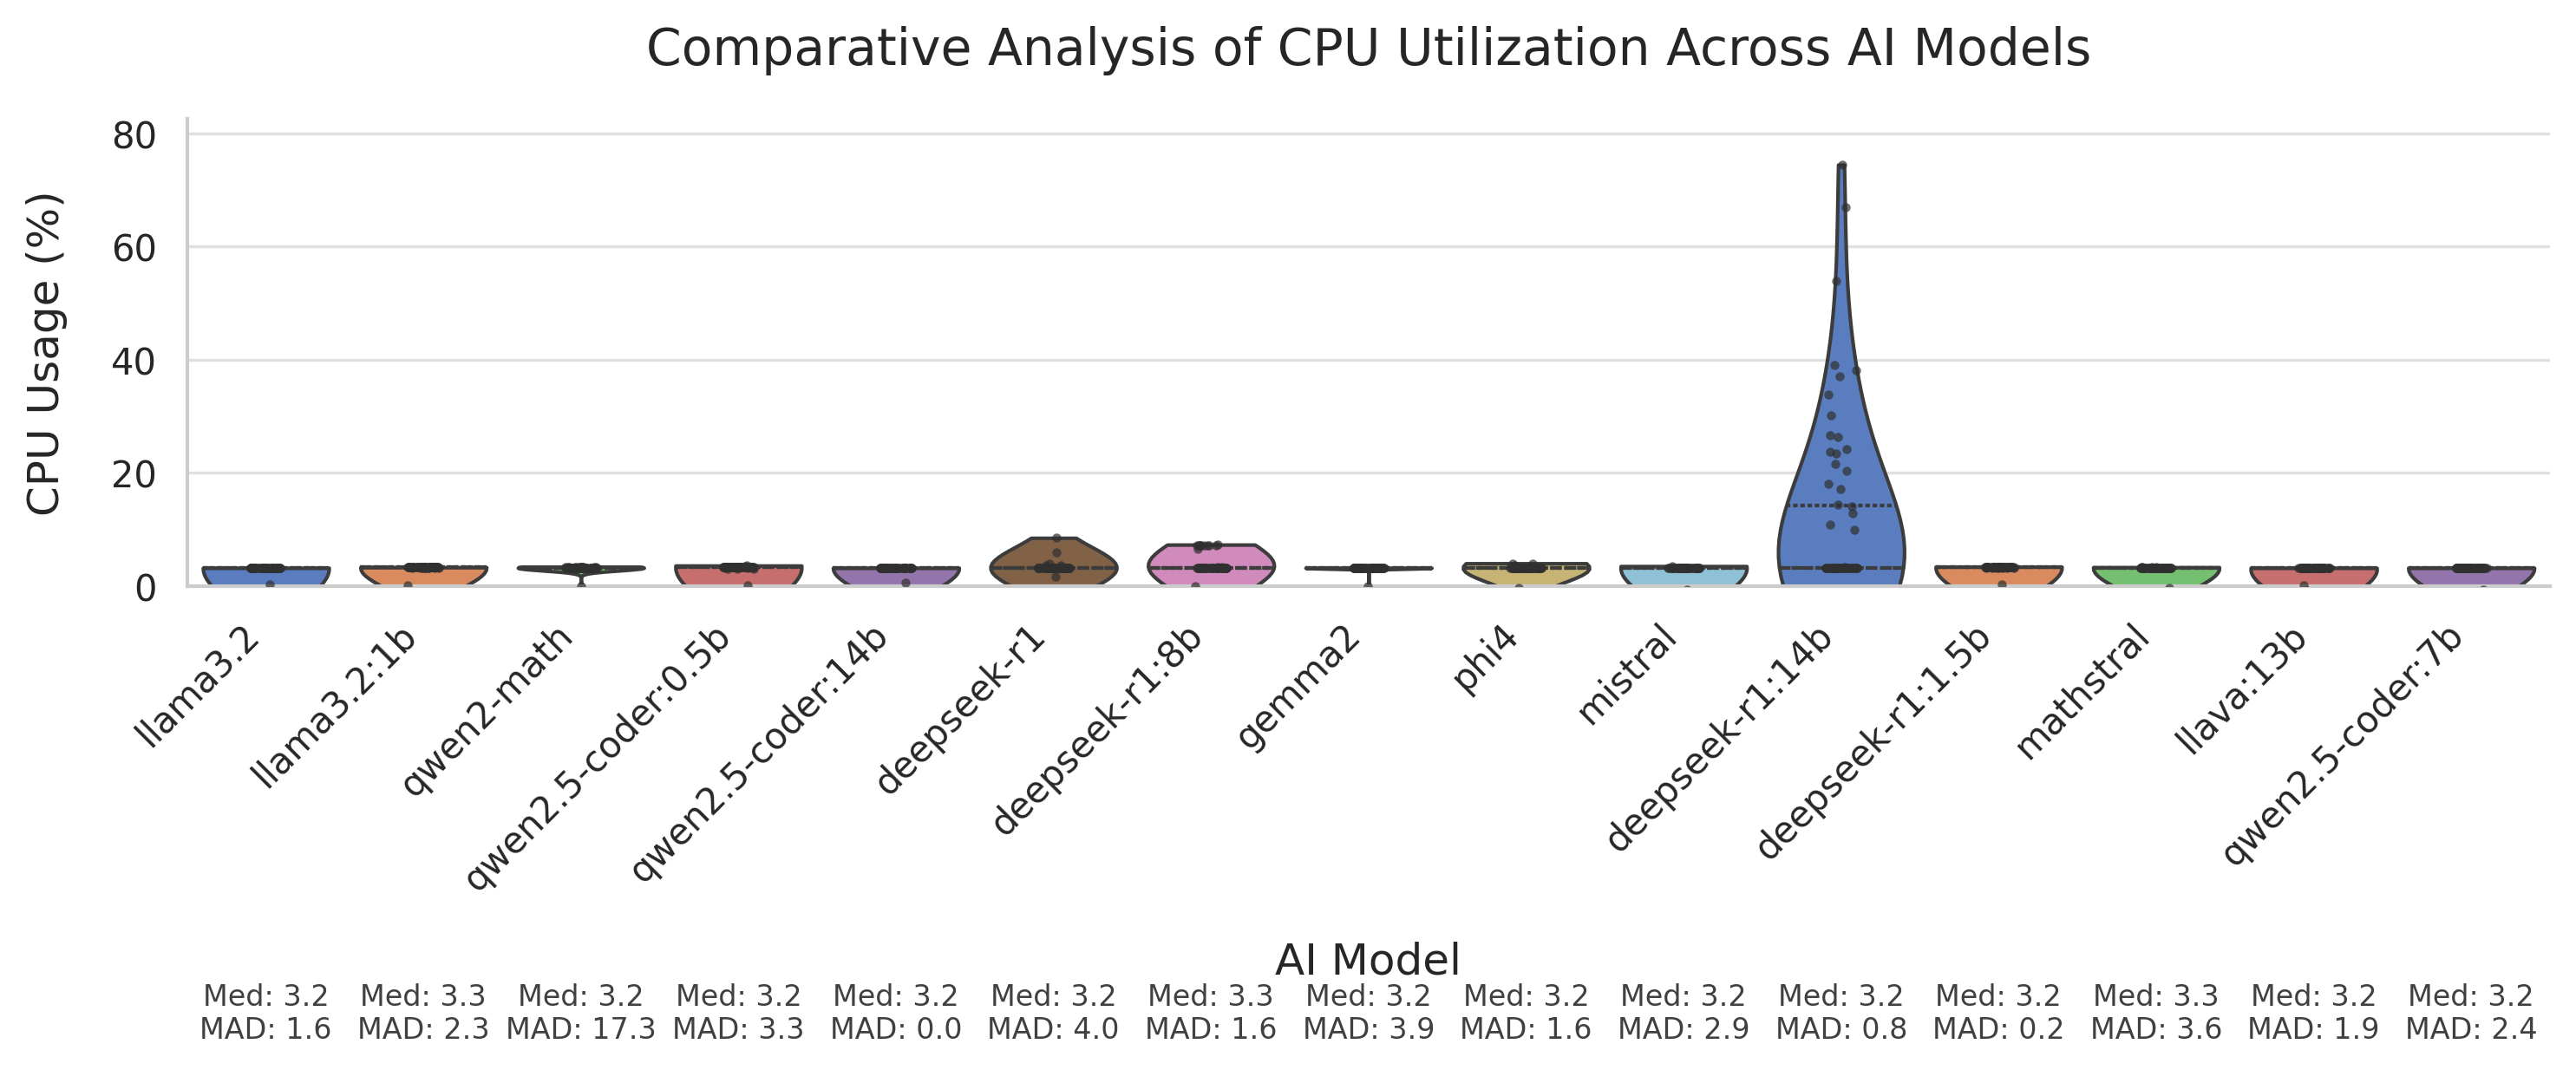
\includegraphics[width=0.8\textwidth]{figures/scores/model_cpu_usage_comparison.png}
  \caption{Comparative Analysis of CPU Utilization Across AI Models}
  \label{fig:cpu_usage_comparison}
\end{figure}

This plot highlights the variability and central tendencies in CPU usage among the evaluated models.

\textbf{Observations:}

CPU usage is relatively consistent across the models; however, the Deepseek (reasoning) models exhibit higher CPU usage, with the largest Deepseek model (14 billion parameters) showing the highest utilization.

\paragraph{Memory Usage}

The following violin plot visualizes the memory consumption of various AI models.

\begin{figure}[H]
  \centering
  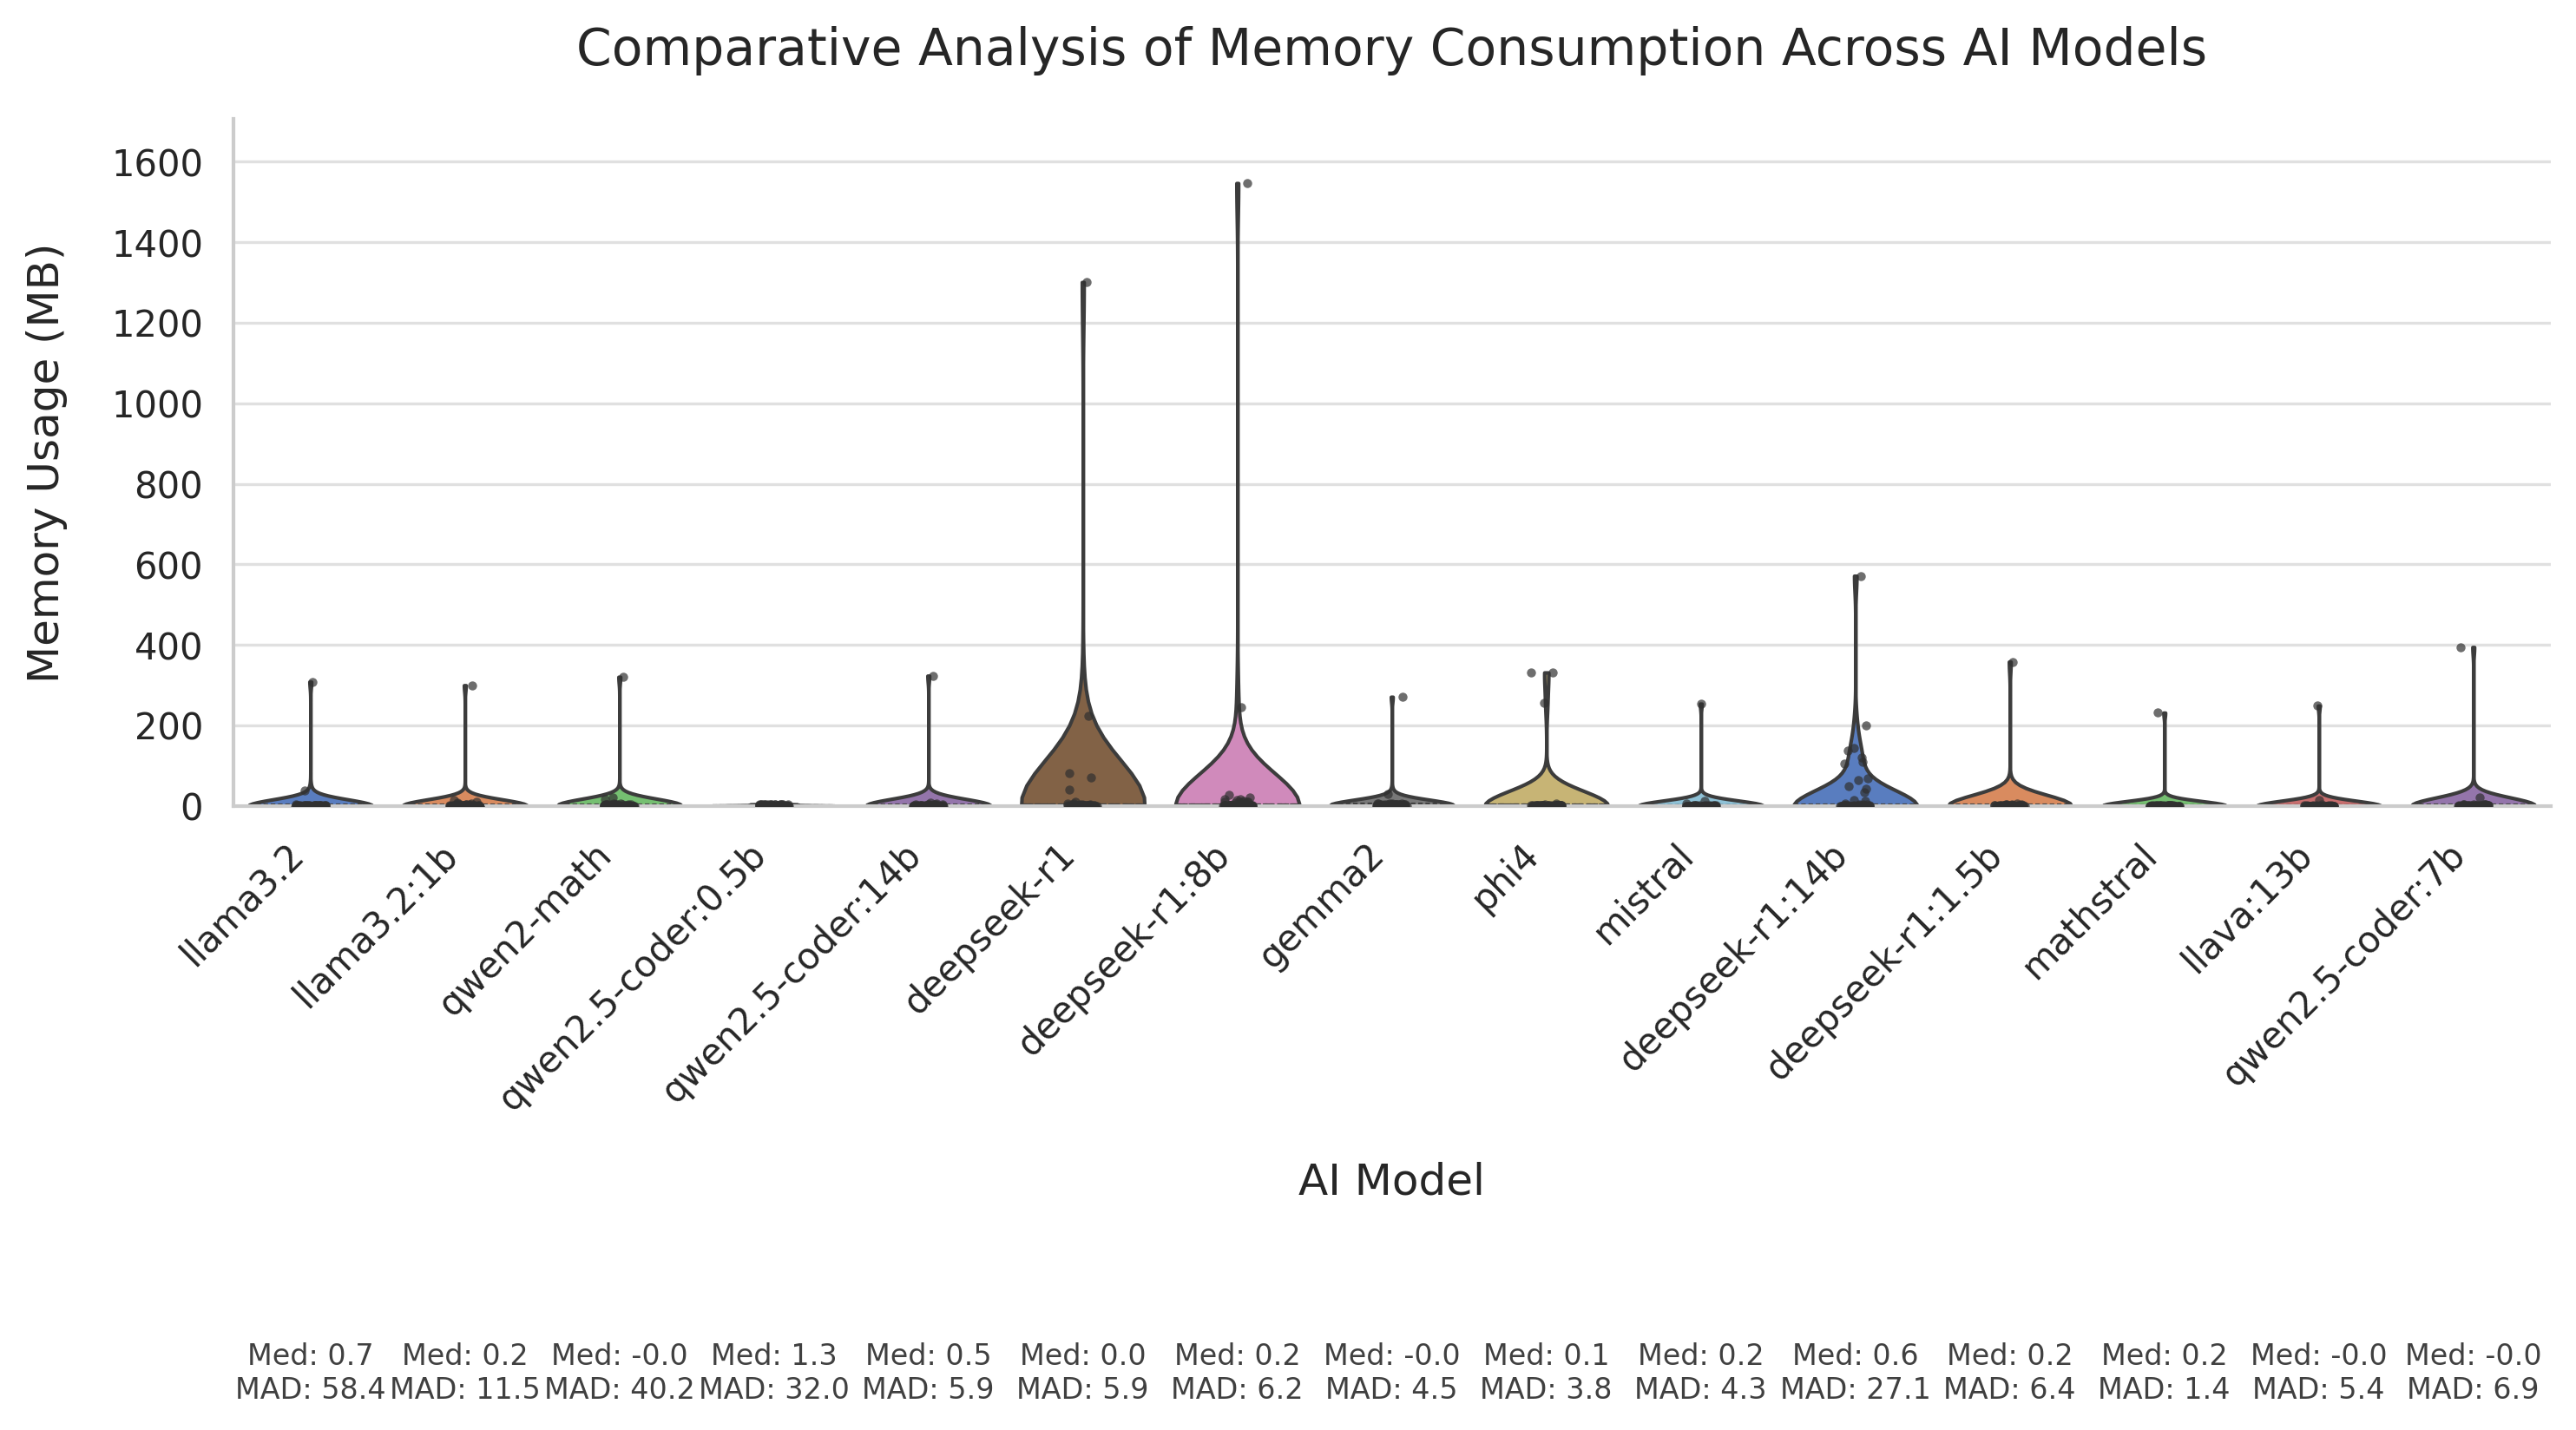
\includegraphics[width=0.8\textwidth]{figures/scores/model_memory_usage_comparison.png}
  \caption{Comparative Analysis of Memory Consumption Across AI Models}
  \label{fig:memory_usage_comparison}
\end{figure}

This visualization reveals the memory usage patterns and distributions, providing valuable insights into resource allocation.

\textbf{Observations:}

Memory usage is generally comparable across the models. Nevertheless, the Deepseek (reasoning) models demonstrate higher memory consumption with a wider spread, particularly in the 8 and 7 billion parameter variants.

\paragraph{Response Times}

A box plot was generated to depict the distribution of response times across the different models.

\begin{figure}[H]
  \centering
  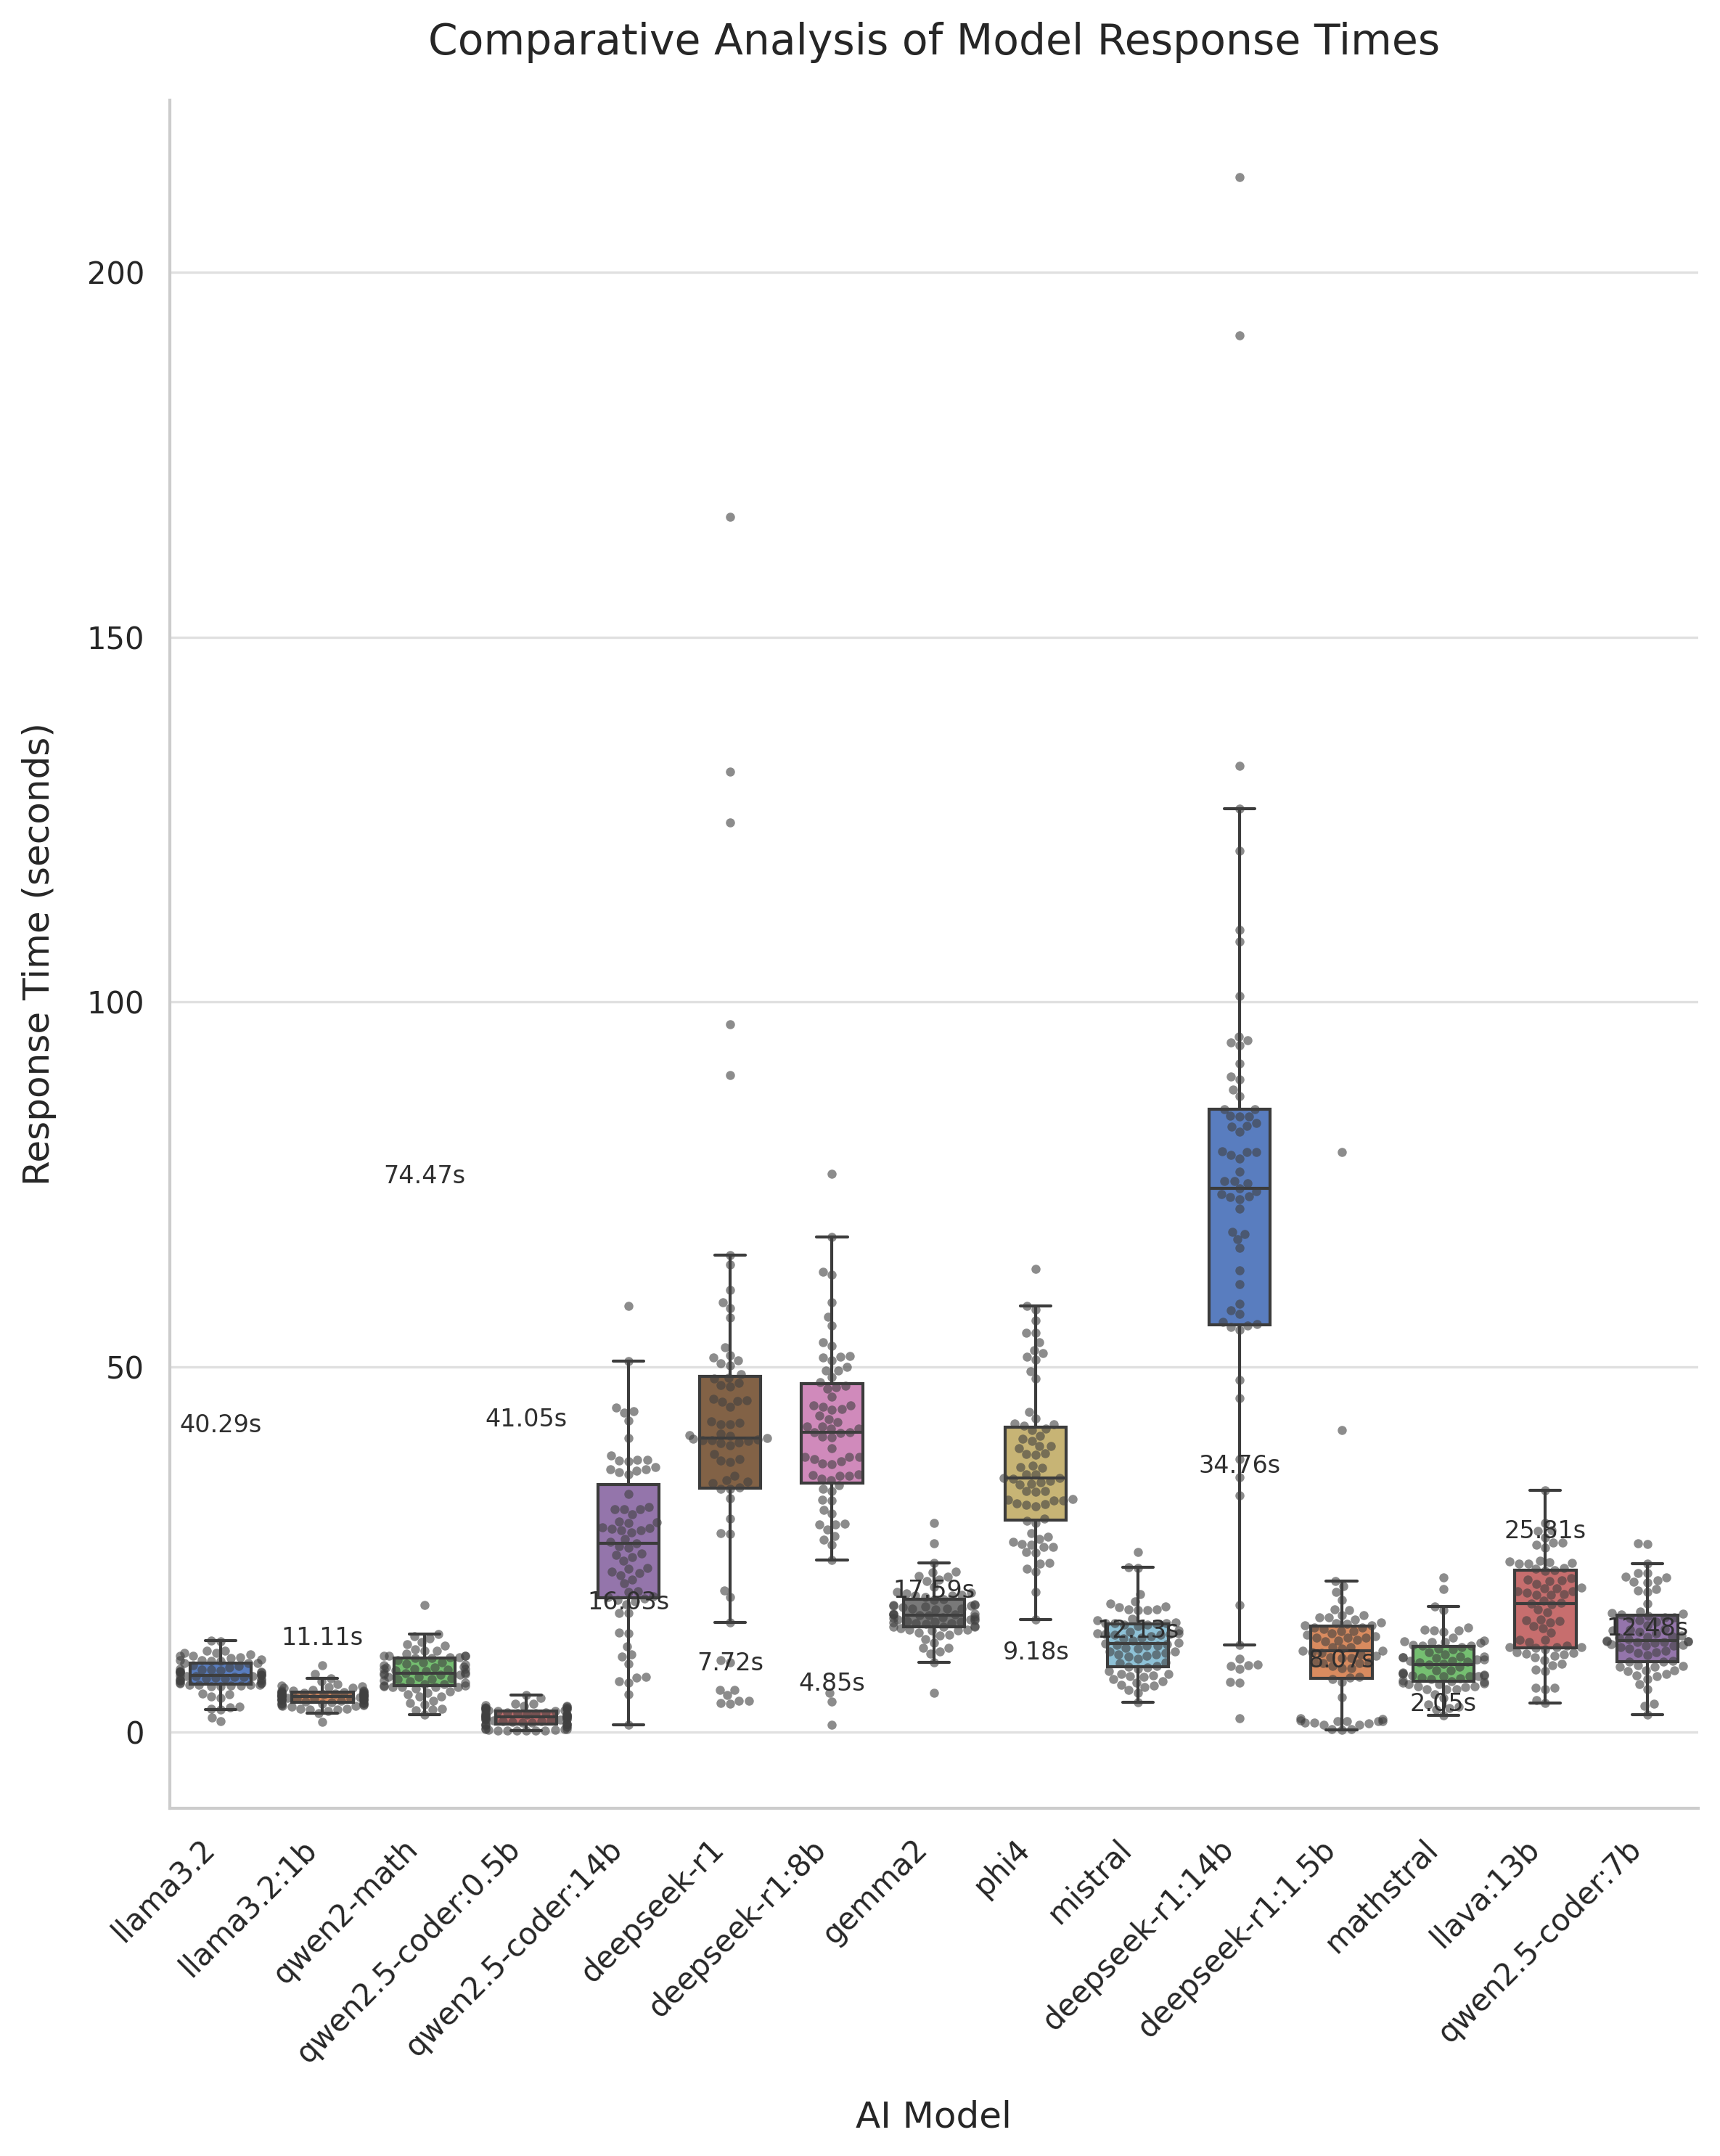
\includegraphics[width=0.8\textwidth]{figures/scores/model_response_times_comparison.png}
  \caption{Comparative Analysis of Model Response Times}
  \label{fig:response_times_comparison}
\end{figure}

This box plot provides a clear overview of the central tendencies and variability in response times.

\textbf{Observations:}

Response times vary significantly among the models. The Llama models display very low and consistent response times, which is advantageous for the intended use case of the School AI Server. In contrast, the Gemma, Mistral, Mathstral, and two Qwen-coder models exhibit higher response times with a noticeable spread. Larger models, such as the Qwen-coder 14 billion parameter model and the Phi4 model, also show increased response times and variability. Notably, the Deepseek models, particularly the 14 billion parameter variant, record the highest response times and spread, likely due to the additional computational demands required for their reasoning processes.

\subsection{Qualitative Data Analysis}

The visualizations presented in this section provide insights into various text quality metrics of different AI models, including BLEU and ROUGE scores, grammatical error counts, readability, and sentiment analysis.

\paragraph{BLEU and ROUGE Scores}

The bar plot below compares the BLEU and ROUGE scores across multiple AI models.

\begin{figure}[H]
  \centering
  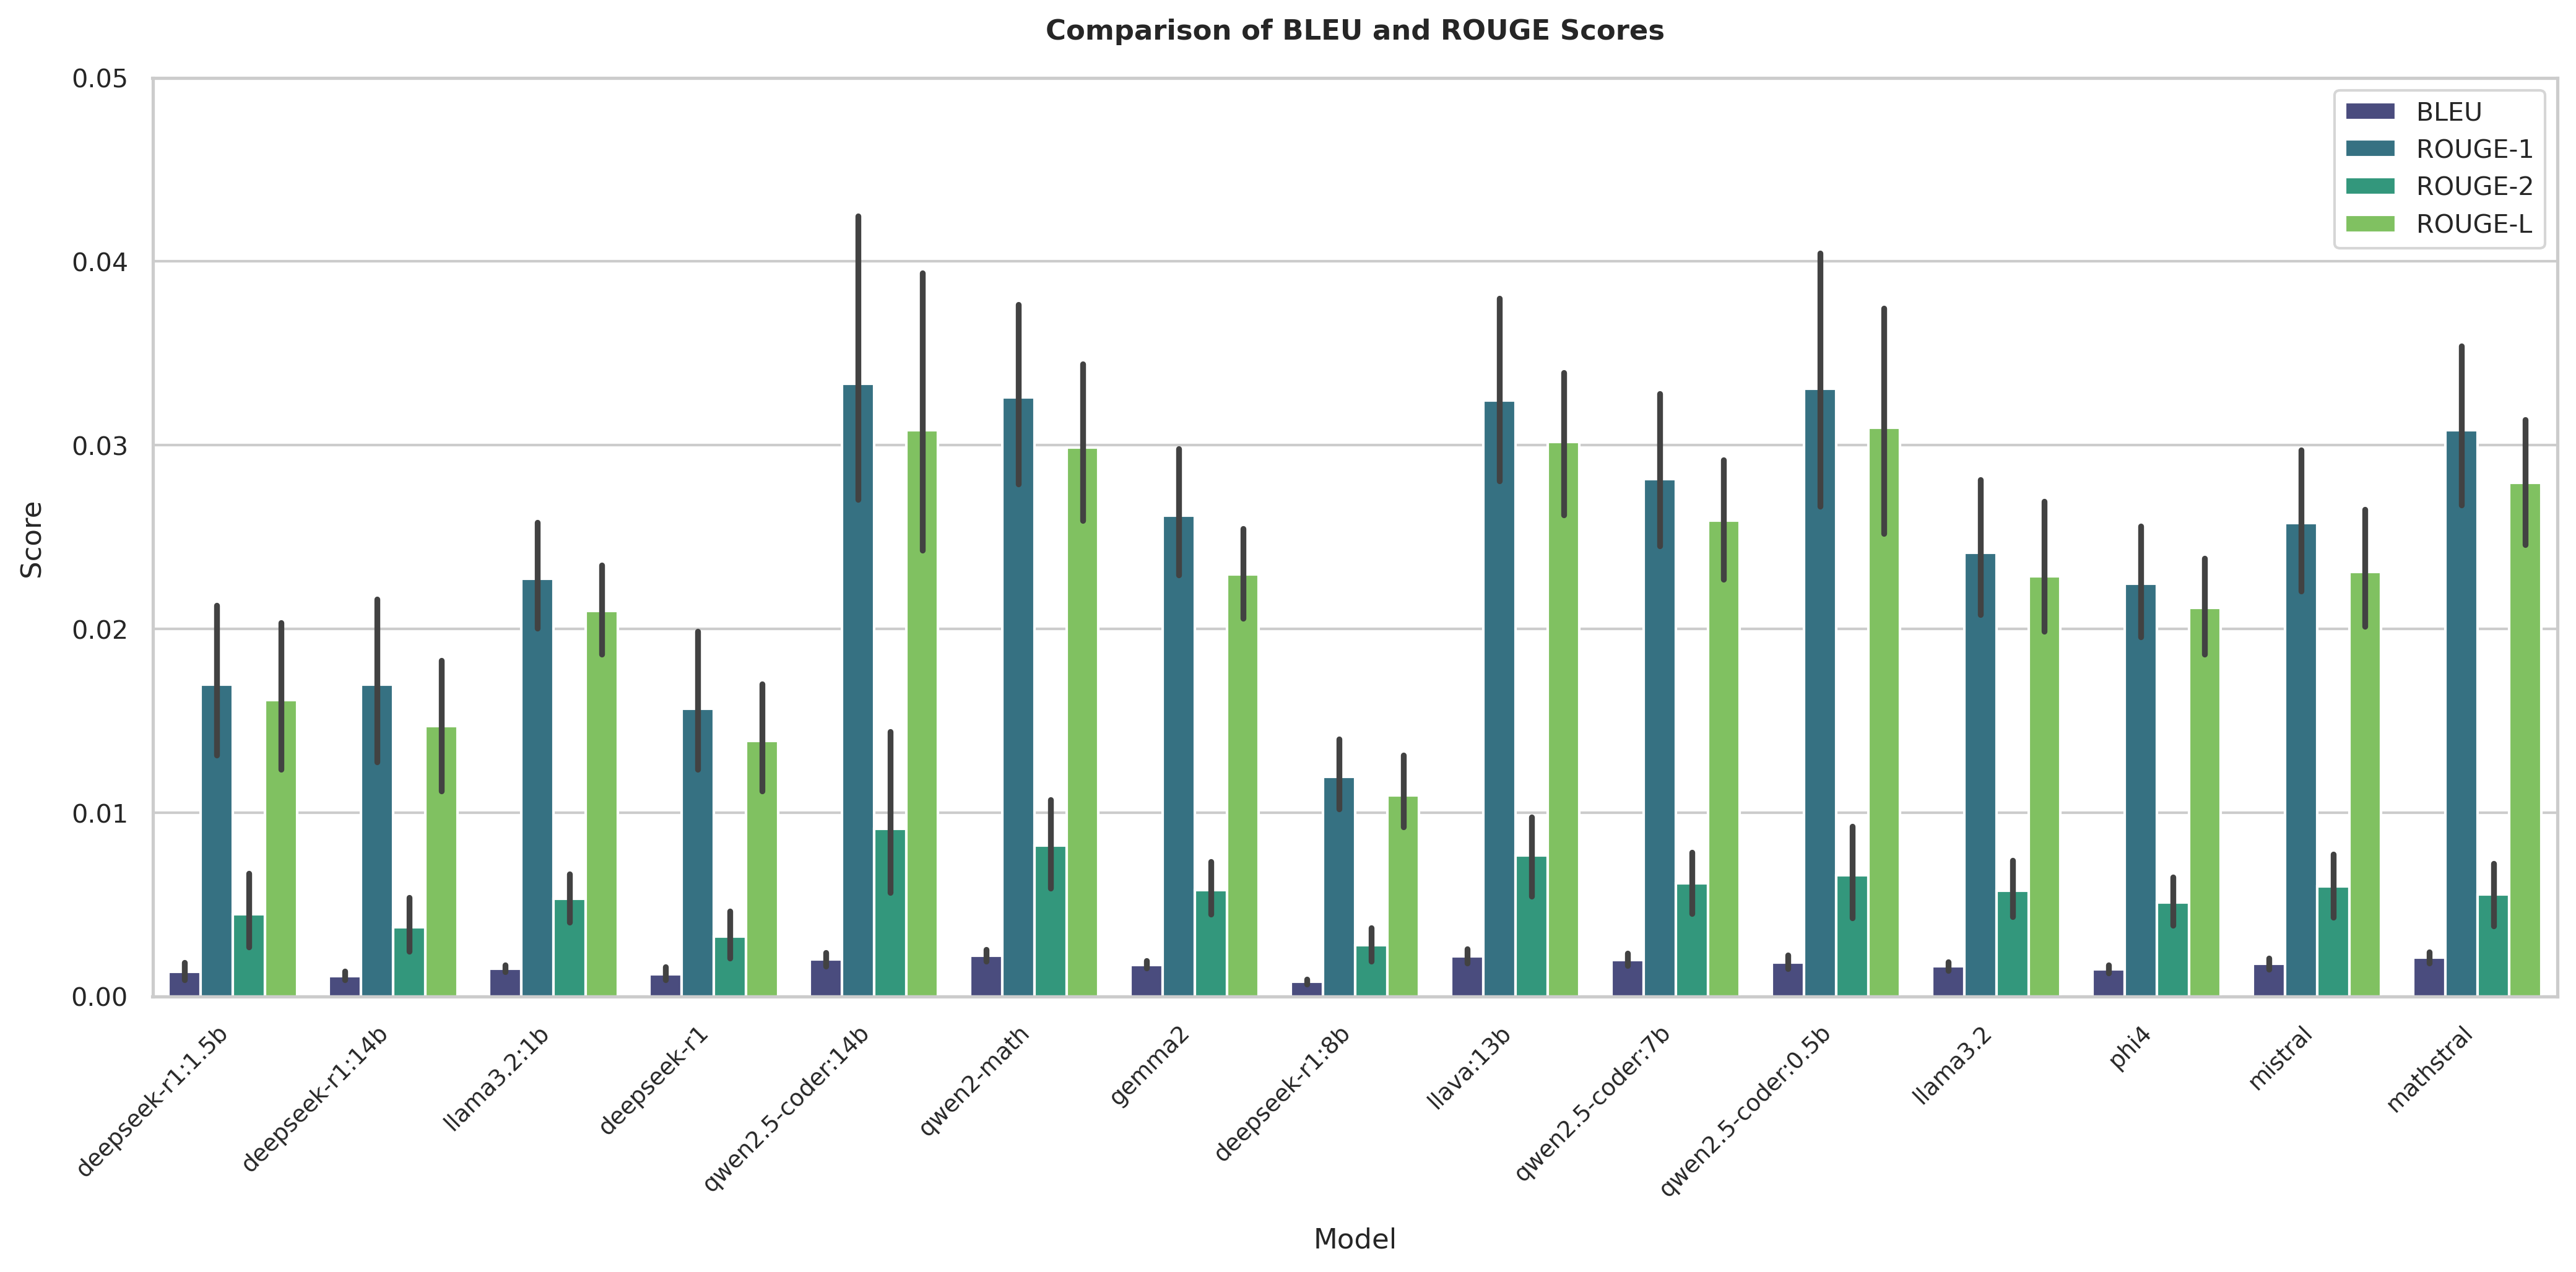
\includegraphics[width=0.8\textwidth]{figures/scores/bleu_rouge.png}
  \caption{Comparison of BLEU and ROUGE Scores}
  \label{fig:bleu_rouge}
\end{figure}

This visualization offers a comprehensive overview of text quality metrics. The BLEU score quantifies the similarity between generated text and a reference text, while the ROUGE scores (including ROUGE-1, ROUGE-2, and ROUGE-L) measure the n-gram overlap between them.

\textbf{Observations:} \\
BLEU and ROUGE scores vary significantly among the models, reflecting differences in text generation quality. Specialized models for mathematics and coding (e.g., Mathstral and Qwen-coder models) achieve the highest scores due to their technical focus. In contrast, general-purpose models such as Llama and Gemma exhibit lower scores, likely as a consequence of their broader but less specialized capabilities. An exception is the Llava model, which—despite being a general-purpose model with vision capabilities—demonstrates a relatively high BLEU score, possibly due to its unique text generation approach based on images. Additionally, the Mistral and Gemma2 models display higher scores among general-purpose models, whereas reasoning models like Deepseek yield the lowest BLEU and ROUGE scores, prioritizing complex logical reasoning over text quality.

\paragraph{Grammatical Errors}

The box plot below illustrates the distribution of grammatical errors detected across different AI models. Grammatical error count serves as an important metric for assessing the linguistic accuracy of generated text. The Language Tool library was used to detect and count errors, with English specified as the target language for consistent and reliable results.\footnote{Note that some errors detected in code snippets were manually corrected to preserve the intended meaning of the visualization.}

\begin{figure}[H]
  \centering
  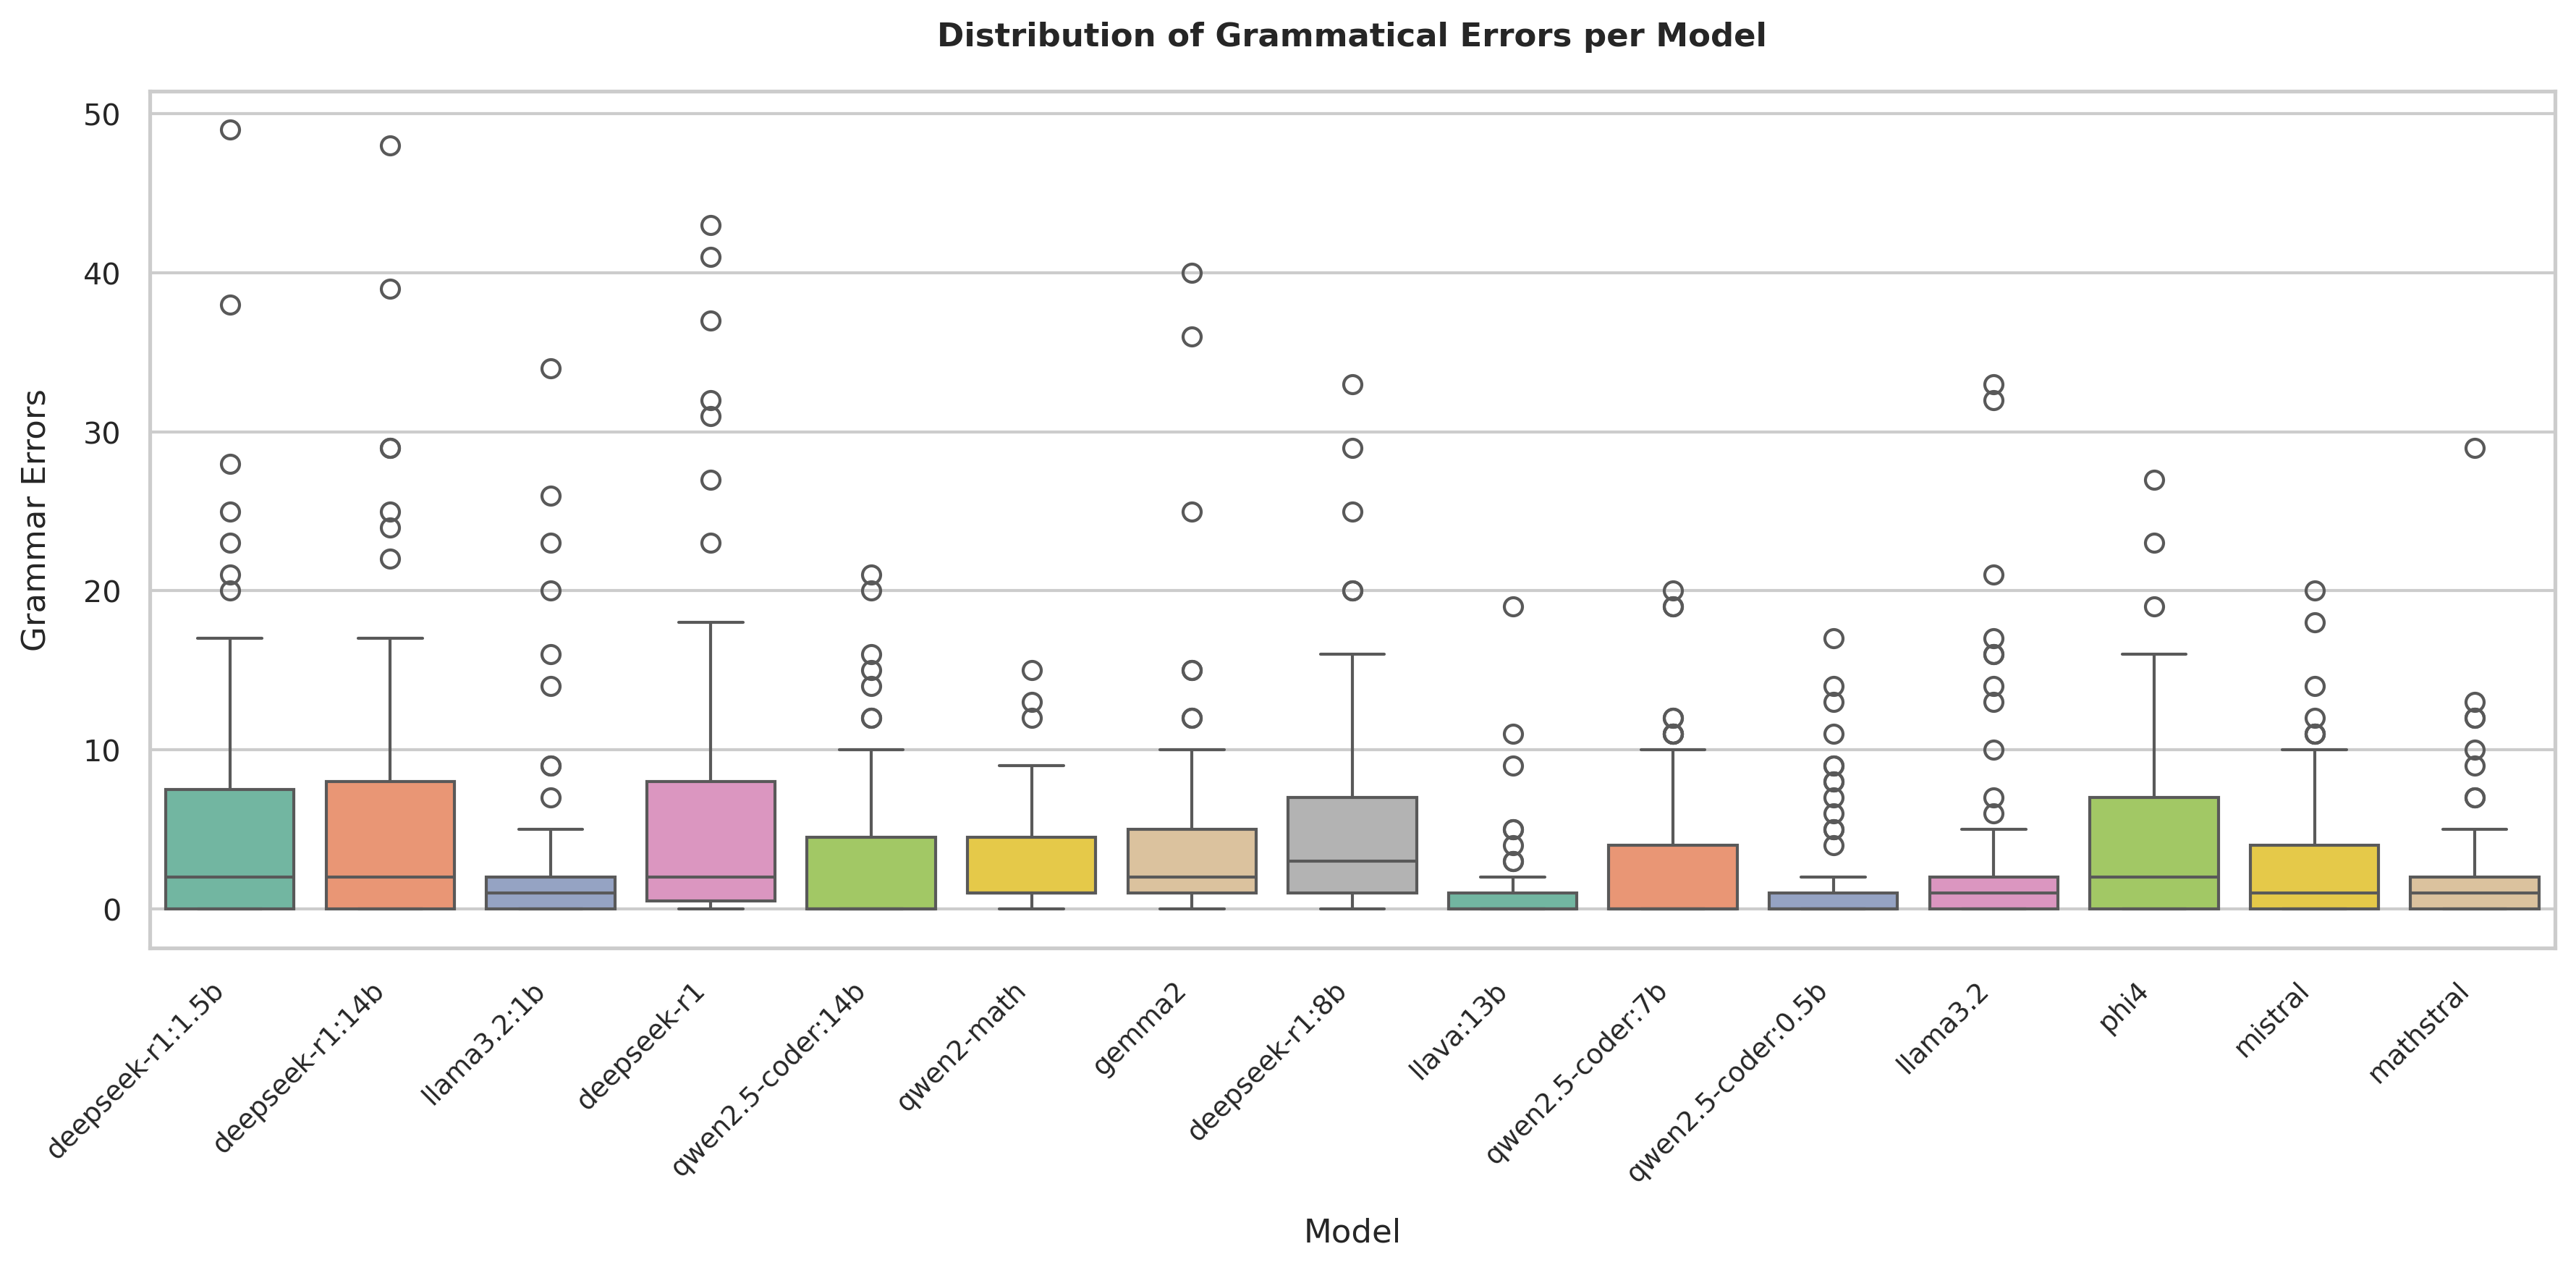
\includegraphics[width=0.8\textwidth]{figures/scores/grammar_errors.png}
  \caption{Comparison of Grammatical Errors Across AI Models}
  \label{fig:grammar_errors}
\end{figure}

\textbf{Observations:} \\
The number of grammatical errors varies considerably between models. The Mathstral, Llava, and Llama models exhibit the fewest errors, with the Qwen-coder models also performing well despite their focus on code generation. In contrast, reasoning models such as Deepseek produce a higher number of errors, which may be attributable to their emphasis on complex logical reasoning rather than linguistic precision. Additionally, some models might generate more errors due to non-native English influences. Notably, the Phi4 model, a general-purpose model developed in the United States, also shows a higher error count.

\paragraph{Readability (Flesch Score)}

The Flesch Reading Ease score quantifies text readability based on the average number of syllables per word and words per sentence. Higher scores indicate more accessible text, while lower scores suggest increased complexity.

\begin{figure}[H]
  \centering
  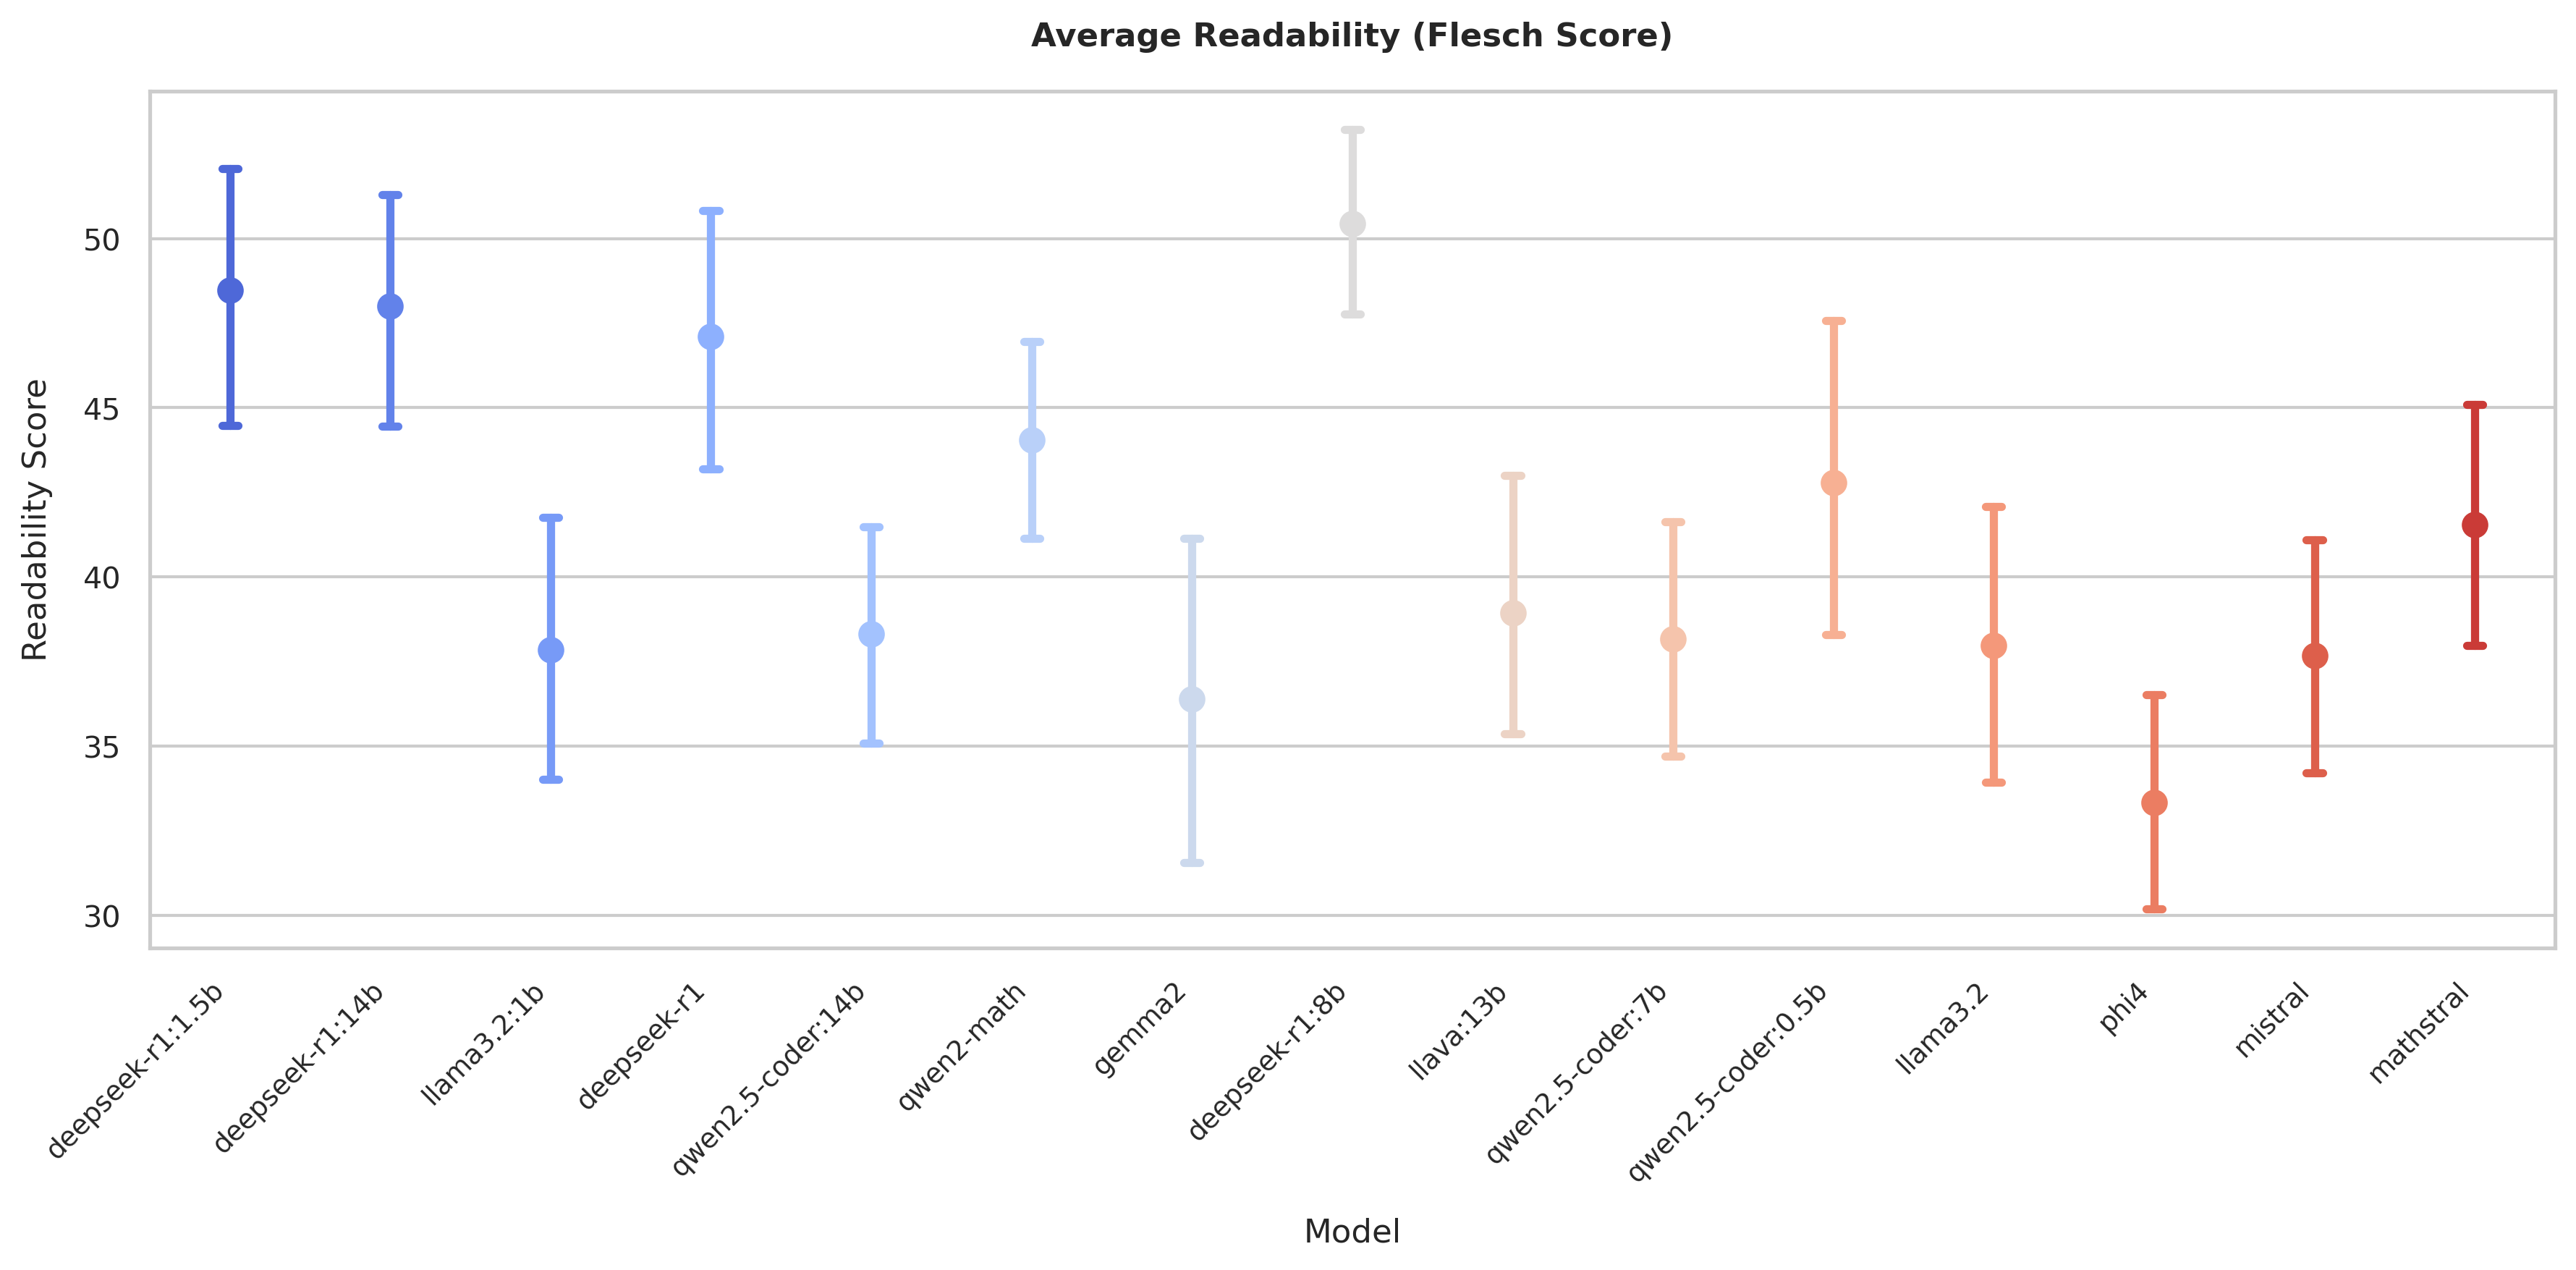
\includegraphics[width=0.8\textwidth]{figures/scores/readability.png}
  \caption{Comparison of Readability Scores Across AI Models}
  \label{fig:readability}
\end{figure}

\textbf{Observations:} \\
Readability scores differ markedly among the models. Interestingly, the Deepseek models achieve the highest readability scores despite their lower BLEU, ROUGE, and grammatical accuracy metrics, possibly due to the nature of their reasoning-focused design. On the other hand, the Gemma2, Phi4, and Llama models score lowest in readability, which is unexpected for general-purpose models that typically aim for accessible language. Specialized models generally fall within the mid-range of readability scores.

\paragraph{Sentiment Analysis}

Sentiment analysis evaluates the emotional tone and polarity of the generated text. A Transformer-based model was employed to classify text as positive or negative.

\begin{figure}[H]
  \centering
  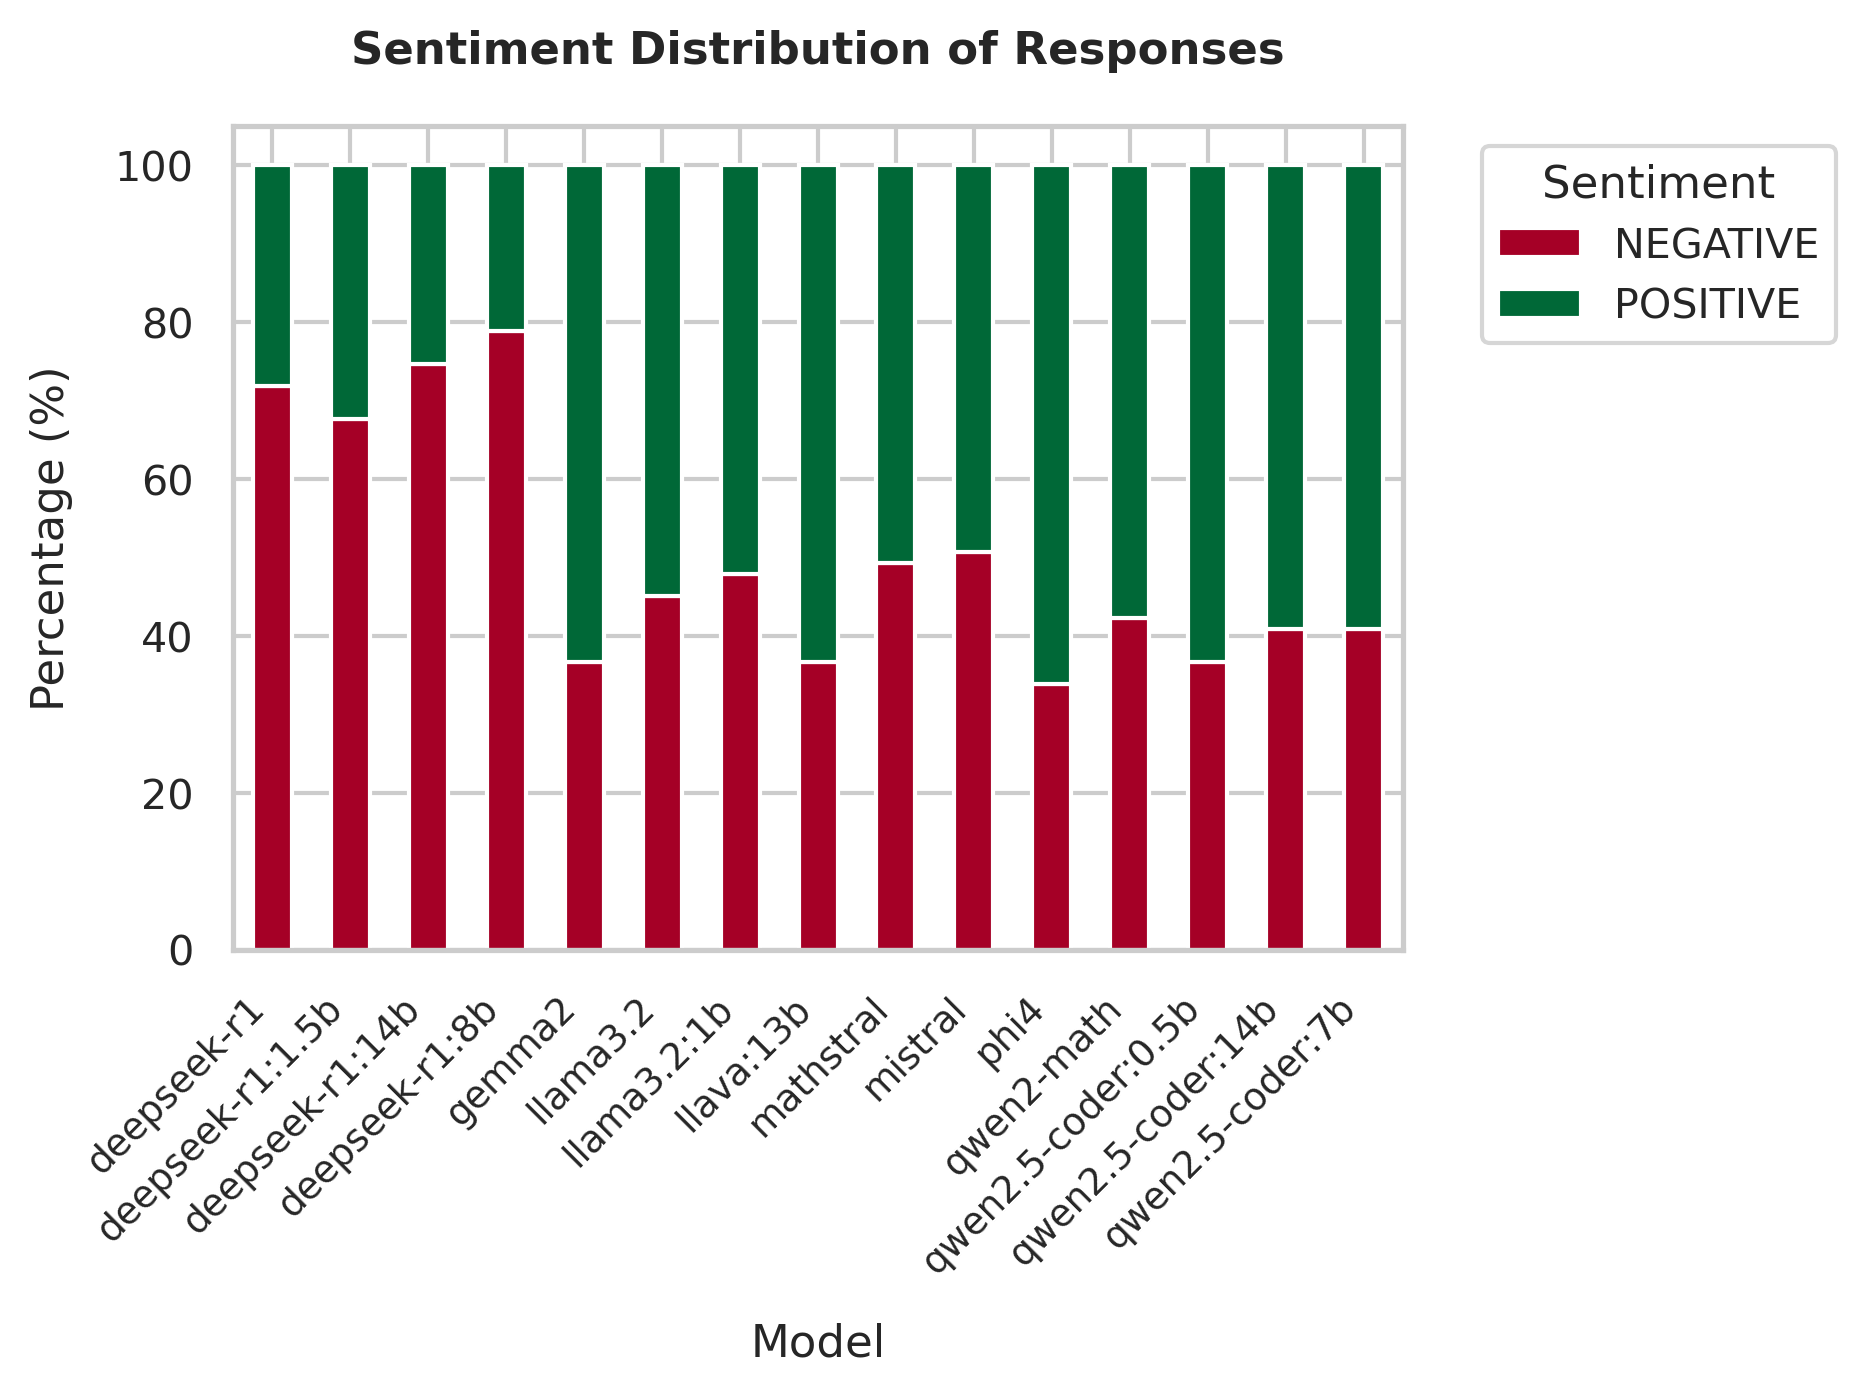
\includegraphics[width=0.8\textwidth]{figures/scores/sentiment.png}
  \caption{Comparison of Sentiment Analysis Across AI Models}
  \label{fig:sentiment}
\end{figure}

\textbf{Observations:} \\
Most models exhibit similar sentiment distributions, with approximately 50–60\% of the text classified as positive and 40–50\% as negative. However, the Deepseek models deviate from this pattern, showing a notably higher negative sentiment score (around 70–80\%), which is intriguing given their high readability scores.

\paragraph{Combined Metrics Overview}

The subplots below provide a holistic overview of the combined text quality metrics, including BLEU and ROUGE scores, grammatical errors, readability, and sentiment analysis.

\begin{figure}[H]
  \centering
  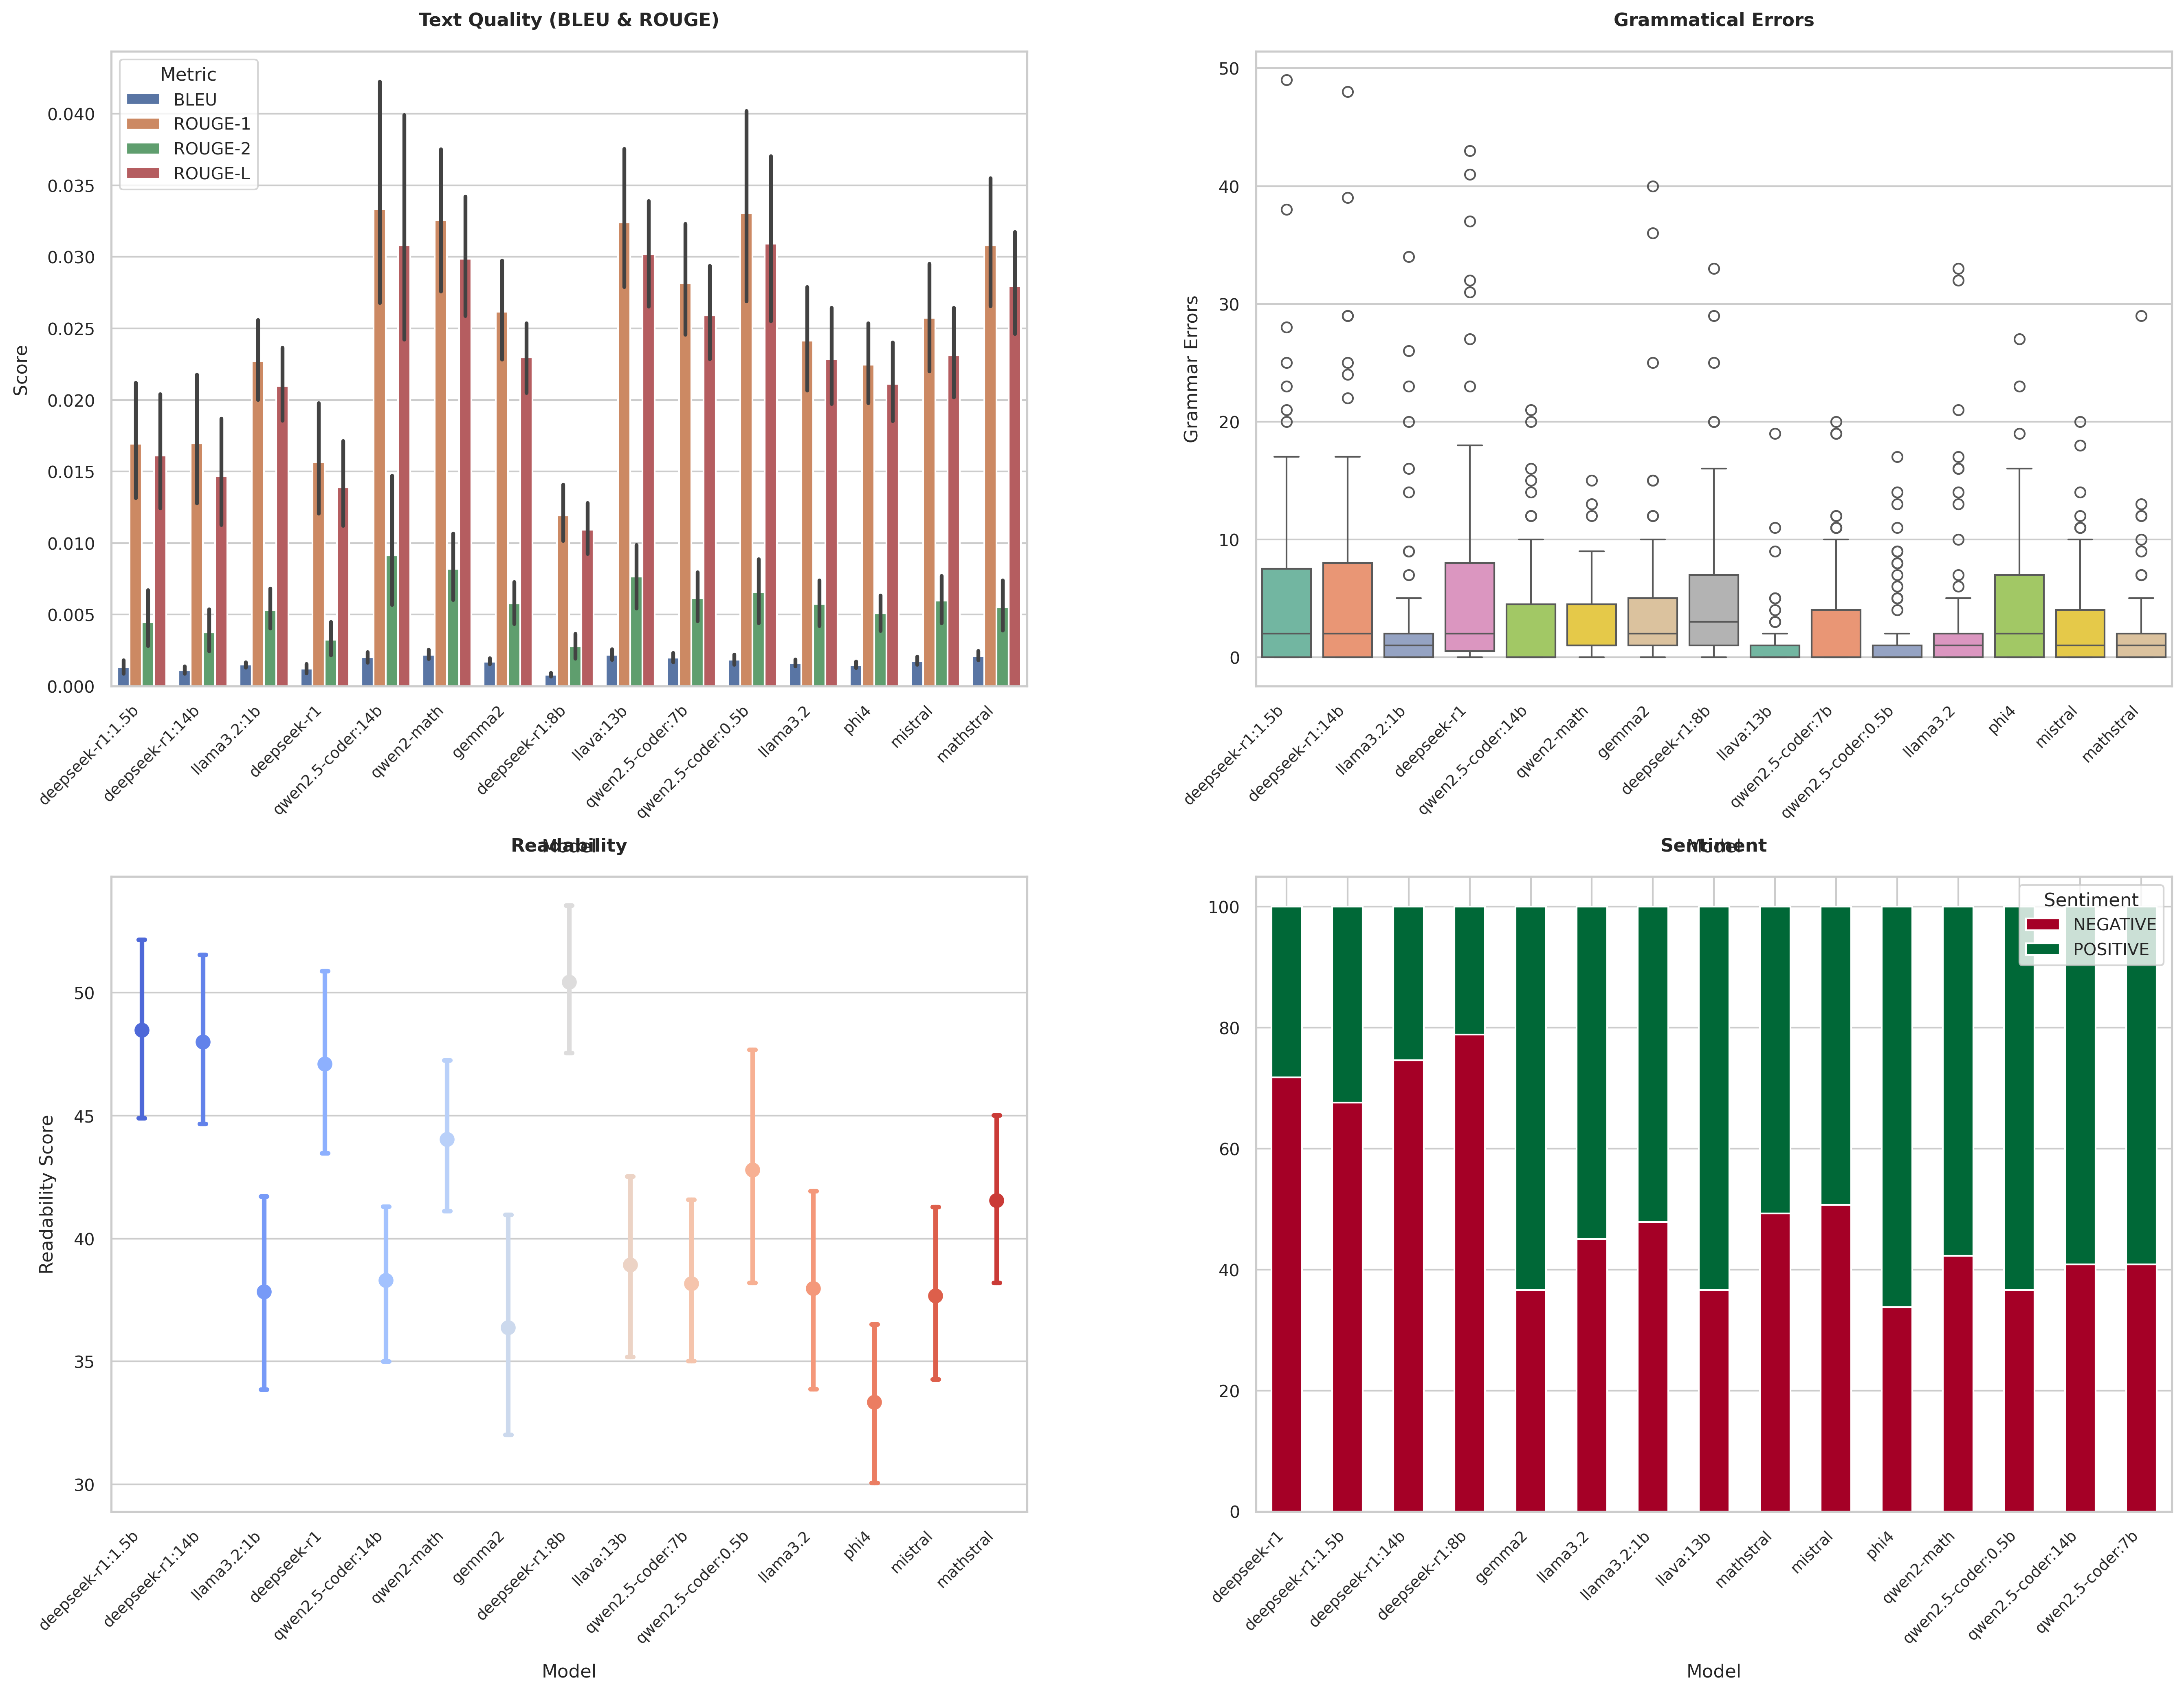
\includegraphics[width=0.8\textwidth]{figures/scores/combined_metrics.png}
  \caption{Combined Metrics Overview for AI Models}
  \label{fig:combined_metrics}
\end{figure}

These subplots facilitate a comprehensive comparative analysis of the performance of different AI models with respect to text quality.


\subsection{Model Comparison for Different Use Cases and Scenarios}

This section presents a comparative analysis of various AI models based on both quantitative and qualitative performance metrics. The evaluation focuses on aspects such as computational efficiency, text generation quality, and overall suitability for specific application scenarios.

\subsubsection{Performance Metrics Overview}

The quantitative analysis reveals significant differences in resource utilization and response times across the models:
\begin{itemize}
  \item \textbf{CPU and Memory Usage:} The Deepseek (reasoning) models tend to exhibit higher CPU and memory consumption compared to others. This is indicative of the increased computational demand required for complex logical processing.
  \item \textbf{Response Times:} Models such as Llama demonstrate very low and consistent response times, making them particularly well-suited for interactive applications. In contrast, larger models (e.g., Qwen-coder 14 billion and Phi4) and the Deepseek models show increased response times and higher variability.
\end{itemize}

\subsubsection{Text Quality and Accuracy}

The qualitative analysis, based on BLEU and ROUGE scores, grammatical error counts, readability, and sentiment analysis, provides further insights into each model's text generation capabilities:
\begin{itemize}
  \item \textbf{BLEU and ROUGE Scores:} Specialized models (e.g., Mathstral and Qwen-coder) achieve the highest scores, reflecting superior performance in generating technical content. General-purpose models like Llama and Gemma tend to score lower due to their broader, less specialized focus.
  \item \textbf{Grammatical Accuracy:} Models such as Mathstral, Llava, and Llama exhibit fewer grammatical errors, while reasoning models like Deepseek show a higher error count, potentially due to their prioritization of logical reasoning over linguistic precision.
  \item \textbf{Readability:} Interestingly, the Deepseek models score highest on the Flesch Reading Ease metric, despite other text quality metrics indicating lower overall quality. In contrast, some general-purpose models such as Gemma2 and Phi4 show lower readability scores.
  \item \textbf{Sentiment Analysis:} Most models present a balanced sentiment distribution. However, the Deepseek models are characterized by a higher proportion of negative sentiment, which may be attributed to the inherent complexity of their reasoning processes.
\end{itemize}

\subsubsection{Use Case Recommendations}

Based on the integrated analysis of both performance and text quality, the following recommendations can be made for various use cases:

\paragraph{Interactive and Real-Time Applications} 
For scenarios requiring rapid response and minimal latency—such as the School AI Server—models like Llama are highly advantageous due to their consistently low response times.

\paragraph{Technical and Domain-Specific Content Generation} 
Applications demanding high accuracy in technical content, particularly in mathematics and coding, are best served by specialized models like Mathstral and Qwen-coder. These models not only achieve superior BLEU and ROUGE scores but also exhibit fewer grammatical errors.

\paragraph{Complex Reasoning Tasks} 
For tasks that necessitate advanced logical reasoning, the Deepseek models are appropriate despite their higher computational resource demands and slower response times. However, users should be aware of the trade-offs, including higher negative sentiment and a greater number of grammatical errors.

\paragraph{General-Purpose Applications} 
For broader applications where versatility is key, general-purpose models such as Gemma, Gemma2, and Phi4 offer a balanced performance. Although they may not excel in any single metric, they provide reliable performance across a range of tasks.

\subsubsection{Overall Evaluation}

The comparative analysis underscores that no single model excels universally across all metrics. Instead, the choice of an AI model should be closely aligned with the specific requirements and constraints of the intended application. Developers must weigh the trade-offs between computational efficiency, text quality, and domain-specific accuracy when selecting the most appropriate model for a given scenario.

\subsection{Model Selected for the Final Application}

For the initial version of the Student AI Hub application, the decision was made to allow users to choose between the models. This approach enables users to select the model that best meets their specific use cases and requirements, while also effectively demonstrating the distinct capabilities of each model.

Specialized models, such as Qwen-coder and LLava, are accessible through dedicated application tabs within the Student AI Hub. In contrast, general-purpose models, including Gemma 2, Phi4, and Llama, are available under the General AI tab.

While reasoning models are available, they have not been fully integrated into the application. Their unique reasoning processes require specialized formatting to ensure that the output is comprehensible to the user. As a result, this formatting was not completely finalized at the time of the initial release of the Student AI Hub.


\subsection{Model Integration and Deployment}

Following the evaluation process, the selected models were systematically integrated into the School AI Server and the Visual Studio Code extension. 

Leveraging the user-friendly API provided by the Ollama application, we facilitated a seamless integration of the models into the School AI Server, ensuring efficient accessibility and deployment. To enhance request management and optimize communication between different components, we developed a Python-based Flask server that hosts a dedicated API. This API serves as an intermediary layer, enabling structured and scalable interactions between the School AI Server and the Visual Studio Code extension.

A comprehensive discussion of the hosted Flask service, including its architecture and functionality, is presented in Chapter 9: \textit{Hosted Flask Service}.


\section{Integration of OpenAI's API}

In this work, we integrated the OpenAI API to leverage proprietary, 
high-performance AI models that are hosted on dedicated servers with advanced hardware capabilities. 
The utilization of external computing power allows for the concurrent execution of multiple models, 
thereby enhancing both scalability and efficiency in our application.

The decision to adopt the OpenAI API was influenced by its widespread adoption, 
robust performance, and extensive documentation. Numerous examples, tutorials, and community resources are available, 
which greatly facilitate the integration process and ensure that best practices are followed in scientific and industrial applications.

\subsection{Overview of the OpenAI API}

The OpenAI API provides access to state-of-the-art AI models developed by OpenAI, including various iterations of the ChatGPT model. 
These models are capable of generating human-like text, answering queries, and engaging in complex conversations. 
The API supports a range of models with different sizes and capabilities, allowing users to select the model that best fits 
the requirements of their specific use cases.

Designed with user accessibility in mind, the API comes with comprehensive documentation and a wealth of code samples, 
which significantly streamline the process of embedding advanced AI functionalities into diverse applications and platforms. 
Furthermore, the API utilizes a token-based pricing model, which charges users according to the number of tokens processed during interactions. 
This pricing structure is not only transparent but also aligns closely with the computational effort required to generate responses.

Before accessing the API's full functionality, users must pre-fund their accounts by depositing a specified amount of money. 
This account-based billing system enables users to manage their expenditures effectively, including the option to set monthly spending limits. 
In addition to text generation, the OpenAI ecosystem also includes DAL-E, an image-generation model that creates visuals based on textual input, 
thus broadening the spectrum of applications available through the API.

\cite{OpenAI-API-Documentation}

\subsubsection{Tokens in Large Language Models}

Tokens are the fundamental units of text that large language models (LLMs) process and generate. 
In this context, a token represents the smallest segment of text that a model can understand, which may correspond to an entire word, 
a fragment of a word, or even an individual character or punctuation mark. 

The process of tokenization involves converting raw text into these discrete units. 
This approach enables LLMs to efficiently capture complex patterns in both syntax and semantics, even when encountering new or out-of-vocabulary terms. 
Techniques such as subword tokenization are particularly valuable, as they break down words into meaningful components, 
thereby reducing the overall vocabulary size and enhancing the model's ability to manage linguistic variability.

Moreover, tokens are closely related to the concept of a context window, which defines the span of tokens a model can consider during text generation or prediction. 
Typically, one token is estimated to average around four characters in English or roughly three-quarters of a word. 
This estimation is crucial for determining computational requirements and understanding the limitations imposed by the model’s finite context window.

In summary, tokens are indispensable for the operation of LLMs, providing a structured means to process language. 
Their effective management through advanced tokenization strategies is essential for optimizing both the computational efficiency and the overall performance 
of these models.

\cite{understanding-tokens-context-window-llms}


\subsection{Data Security and Privacy in Compliance with Austrian and EU Regulations}
\label{sec:data-security-privacy-openai}

The integration of OpenAI's API into our systems necessitates a comprehensive examination of data security and privacy, 
particularly with regard to compliance with both Austrian and European Union regulatory frameworks. 
In this context, our approach adheres to the stringent requirements set forth in Regulation (EU) 2016/679
(General Data Protection Regulation, GDPR) \cite{EU2016GDPR}, which forms the cornerstone of data protection within the EU. Additionally,
the relevant provisions of the Austrian Data Protection Act (Datenschutzgesetz DSG) \cite{AustrianDSG} have been carefully 
to ensure that personal data is handled in accordance with national standards.

OpenAI has implemented several measures to safeguard user data and align with GDPR mandates. 
Notably, they support compliance with privacy laws such as the GDPR and the California Consumer Privacy Act (CCPA), 
offering a Data Processing Addendum to customers. Their API and related products have undergone evaluation by an independent third-party auditor, 
confirming alignment with industry standards for security and confidentiality. 

\cite{OpenAI-Data-Residency-Europe}

Despite these measures, concerns have been raised regarding data handling practices. 
For instance, data transmitted through the OpenAI API could potentially be exposed, and compliance with GDPR remains a complex issue. Additionally, 
data may be accessible to third-party subprocessors, introducing further privacy considerations.

\cite{OpenAI-privacy-complaint-Austria}

To address these concerns, we have proactively informed our user community through a notice on the school website. 
This notice outlines the data handling practices associated with the OpenAI API and provides guidance on how users can manage their data when 
interacting with our systems. By maintaining transparency and offering clear instructions, 
we aim to uphold the highest standards of data security and privacy in our school environment.

In light of the evolving regulatory landscape, it is important to remain vigilant and responsive to any changes in data protection laws within 
Austria and the broader EU. Continuous monitoring and adaptation of our data handling practices will ensure ongoing compliance and the safeguarding of user privacy. 


\subsection{OpenAI API Implementation in Vue.js}
\label{sec:openai-api-implementation}
This section details the integration of the OpenAI API within a Vue.js application framework, with a focus on both text and image generation capabilities. The implementation not only illustrates the interaction between the Vue.js frontend and the OpenAI API but also demonstrates adherence to security best practices and modular code design. The following discussion is supported by annotated code examples and an explanation of the libraries used.

\subsubsection{Overview of the Implementation}

The implementation is structured as a Vue.js component that facilitates the following functionalities:
\begin{itemize}
    \item Accepting user input via a text area.
    \item Initiating API calls for generating text responses (using ChatGPT models) and creating images (via the DALL-E endpoint).
    \item Displaying the results (generated text and images) dynamically within the user interface.
\end{itemize}

The component is designed with a clear separation between presentation and business logic, ensuring that the code remains both maintainable and scalable.

\subsubsection{Explanation of the Used Libraries}

\paragraph{OpenAI Library}  
The library is employed as the primary interface to interact with OpenAI’s API endpoints. This library abstracts the complexities of HTTP communication and provides a user-friendly API to access advanced AI functionalities such as natural language generation and image synthesis. Its integration simplifies the process of constructing API requests and handling responses, which is critical for developing robust AI-driven applications.

\paragraph{API Key Management}  
To ensure secure handling of sensitive credentials, the OpenAI API key is imported from an external module (i.e., \texttt{OPENAI\_API\_KEY} from the \texttt{secrets} file). This approach adheres to security best practices by preventing the direct embedding of API keys within the source code, thereby mitigating the risk of unauthorized exposure.

\subsubsection{Code Example: Vue.js Component for OpenAI API Integration}

Below is an illustrative example of a Vue.js component that integrates the OpenAI API for both text and image generation. The code is presented in two parts: the HTML template and the JavaScript logic.

\paragraph{HTML Template}
\begin{lstlisting}[language=HTML, caption=Vue.js Template for OpenAI API Integration]
<template>
  <div class="openai-container">
    <h1>OpenAI API Integration in Vue.js</h1>
    <textarea 
      v-model="userInput" 
      placeholder="Enter your prompt here..." 
      rows="4" 
      cols="50">
    </textarea>
    <div class="action-buttons">
      <button @click="generateText">Generate Text</button>
      <button @click="generateImage">Generate Image</button>
    </div>
    <div v-if="generatedText" class="output-section">
      <h2>Generated Text</h2>
      <p>{{ generatedText }}</p>
    </div>
    <div v-if="generatedImage" class="output-section">
      <h2>Generated Image</h2>
      <img :src="generatedImage" alt="Image generated by OpenAI API" />
    </div>
  </div>
</template>
\end{lstlisting}

\paragraph{JavaScript Logic}


\begin{lstlisting}[language=JavaScript, caption=Vue.js Script for OpenAI API Integration]
<script>
import OpenAI from "openai";
import { OPENAI_API_KEY } from "../secrets";

export default {
  name: "OpenAIComponent",
  data() {
    return {
      userInput: "",
      generatedText: "",
      generatedImage: ""
    };
  },
  methods: {
    async generateText() {
      // Initialize OpenAI client with API key
      const openai = new OpenAI({ apiKey: OPENAI_API_KEY });
      try {
        const response = await openai.chat.completions.create({
          model: "gpt-3.5-turbo",
          messages: [{ role: "user", content: this.userInput }]
        });
        // Extract and assign the generated text
        this.generatedText = response.choices[0].message.content;
      } catch (error) {
        console.error("Error during text generation:", error);
      }
    },
    async generateImage() {
      // Initialize OpenAI client for image generation
      const openai = new OpenAI({ apiKey: OPENAI_API_KEY });
      try {
        const response = await openai.images.generate({
          prompt: this.userInput,
          n: 1,
          size: "512x512"
        });
        // Extract and assign the URL of the generated image
        this.generatedImage = response.data[0].url;
      } catch (error) {
        console.error("Error during image generation:", error);
      }
    }
  }
};
</script>
\end{lstlisting}

\subsubsection{Discussion}

The presented component exemplifies how modern web applications can seamlessly integrate AI capabilities while maintaining a secure and modular architecture. Key points of consideration include:
\begin{itemize}
    \item \textbf{Modularity:} The separation of the UI (HTML template) and the business logic (JavaScript methods) facilitates easier maintenance and potential scalability.
    \item \textbf{Security:} By importing the API key from an external secrets module, the risk of credential leakage is minimized. This practice is crucial in academic and production environments where data security is paramount.
    \item \textbf{Extensibility:} The design allows for further expansion, such as additional error handling mechanisms or the integration of more advanced functionalities provided by the OpenAI API.
\end{itemize}

In conclusion, this integration not only demonstrates the practical application of AI APIs in modern web development but also reflects best practices in secure and maintainable code design. Such an approach is essential for building reliable applications in both academic research and industrial contexts.


\section{Conclusion}

The comprehensive evaluation of AI models for the Student AI Hub application has yielded valuable insights into their performance across various metrics, including response times, resource utilization, text quality, and overall suitability for diverse use cases. By integrating both quantitative and qualitative analyses, we have identified the strengths and weaknesses of each model, enabling us to formulate informed recommendations tailored to specific application scenarios.

Furthermore, the integration of the OpenAI API into the School AI Server and the Visual Studio Code extension has significantly enhanced the application's capabilities, providing users with seamless access to advanced AI functionalities. Adherence to best practices in data security and privacy has ensured full compliance with Austrian and EU regulations, thereby safeguarding user data.

In the following three chapters, we will discuss the technical implementation aspects of the project, including the integration of AI into the Flask server, the development of the Student AI Hub application, and the incorporation of AI functionalities into the Visual Studio Code extension. These chapters will provide a detailed exploration of the project's technical architecture, complete with code examples, architectural diagrams, and deployment strategies.








